\documentclass[journal]{IEEEtran}

\usepackage{graphicx}
\usepackage{booktabs}
\usepackage{amsmath,amssymb}
\usepackage{url}

\newcommand{\Rc}{R_{\mathrm{c}}}
\newcommand{\Rs}{R_{\mathrm{s}}}

\begin{document}

\title{Supplementary Material for ``ISAC-Assisted Topology-Aware Narrow-Beam Neighbor Discovery for Distributed-Execution UAV Swarms''}

\author{Author~Names~Omitted~for~Anonymous~Review}

\maketitle

\section{Scope of This Supplement}

This supplement records the experiment coverage and stress evidence supporting the bounded claims in the main manuscript.
The main paper should be read as a cross-layer link-layer neighbor-discovery study: ISAC provides an imperfect beam-cell occupancy prior, and neighbor edges are created only by bidirectional narrow-beam handshakes.
The additional figures and tables below are used to bound the claims rather than to assert universal robustness.

\section{Experiment Coverage}

Table~\ref{tab:supp_coverage} maps the main reviewer-facing experiment requirements to archived artifacts.
The complete evidence map is maintained in the repository coverage matrix.

\begin{table*}[!t]
  \centering
  \caption{Coverage of Requested Experiment Dimensions}
  \label{tab:supp_coverage}
  \scriptsize
  \setlength{\tabcolsep}{3pt}
  \begin{tabular}{p{0.17\textwidth}p{0.12\textwidth}p{0.38\textwidth}p{0.16\textwidth}}
    \toprule
    Requirement & Status & Primary artifacts & Boundary \\
    \midrule
    Beamwidths 3--30 deg & Main+stress & Main 5/10/15/30 deg: round3 N=100 transfer/robustness tables; stress 3/5/10/15/30 deg: round7 scale-beam grid; full 3 deg five-baseline check: round9. & 3 and 5 deg are stress regimes. \\
    Node counts 10--100 & Partially crossed & Round7 scale-beam grid and round3 N=100 density/fixed scaling. & Not a full Cartesian cross with every mobility and error setting. \\
    Small-to-large transfer & Bounded & Training at $N=10$, 10 deg; N=100 zero-shot tables and figures. & Main training is shared-parameter protocol tuning. \\
    Baselines & Main+stress & Uniform random, SkyOrbs-like, learned no-ISAC, enhanced no-ISAC, enhanced ISAC. & SkyOrbs-like is not a full SkyOrbs reproduction. \\
    Mobility models & Boundary & Round5 main mobility, round7 mobility stress, round8 missing-baseline table. & Abrupt mobility remains a boundary. \\
    Range and timing & Sensitivity & Range grid and slot-duration sensitivity. & Protocol-level abstraction, not calibrated RF range law. \\
    ISAC errors & Configured & B=10 main error profiles, B=15 Gauss-Markov/random-walk extension. & Does not imply estimator immunity. \\
    Training curves & Trace & Round2 and round7 reward and score histories. & Empirical training-score evolution only. \\
    \bottomrule
  \end{tabular}
\end{table*}

\section{Training and Scale Transfer Evidence}

Fig.~\ref{fig:supp_training} reports the empirical reward and score evolution of the shared-parameter policy-search run used to select the candidate learned policy.
The curves are not used as a proof of convergence; they document that the selected policy came from a stabilized training-score region rather than from a single isolated episode.

\begin{figure*}[!t]
  \centering
  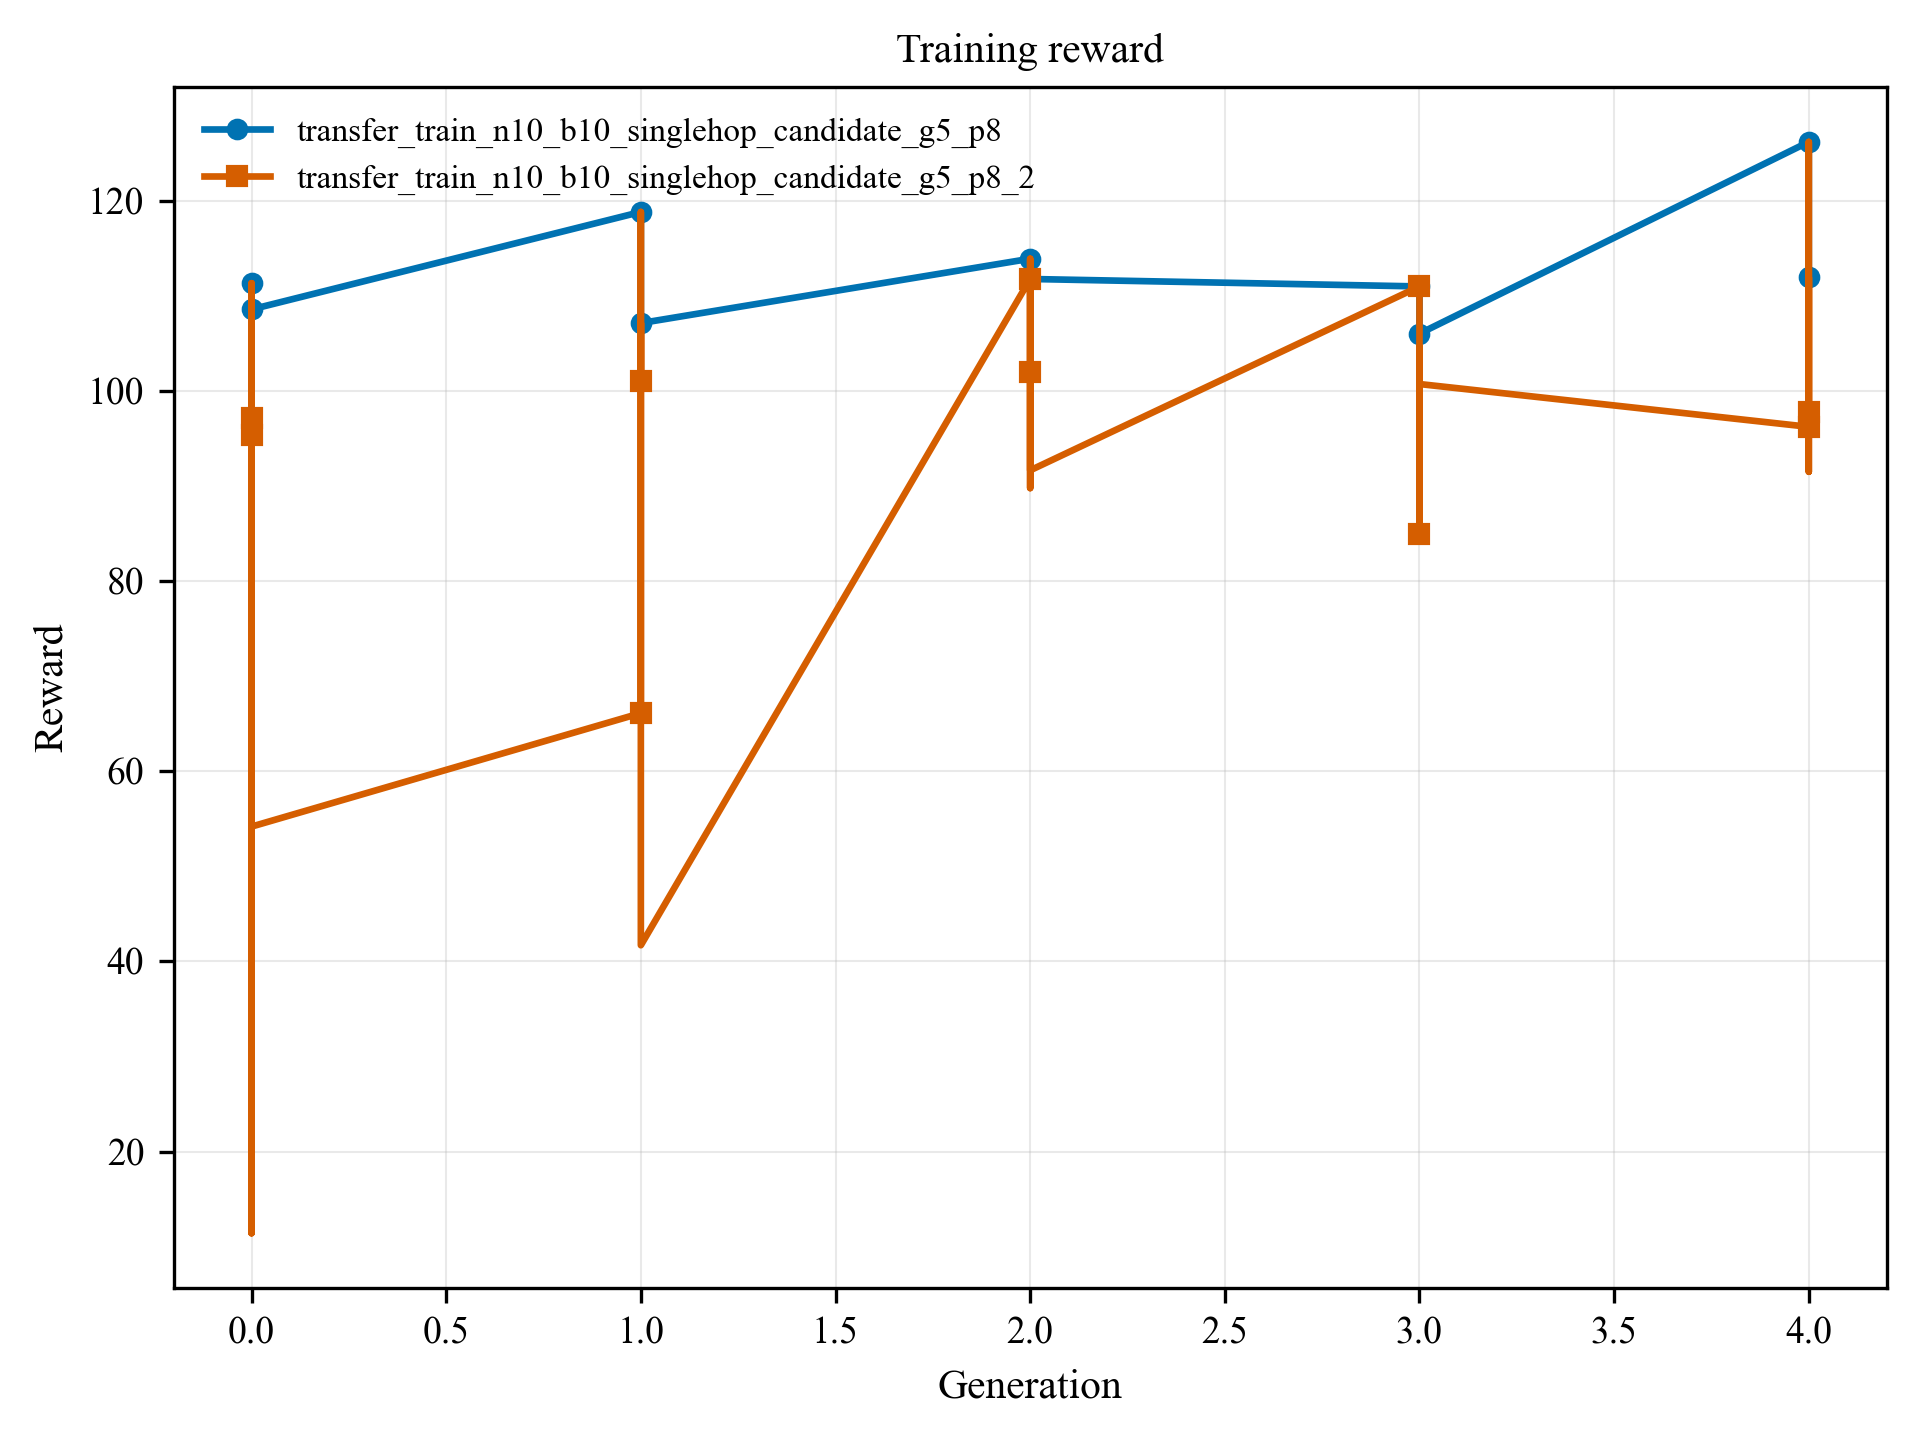
\includegraphics[width=0.48\textwidth]{../../06_analysis/paper_figures/training_round2_candidate/train_reward_curve.png}
  \hfill
  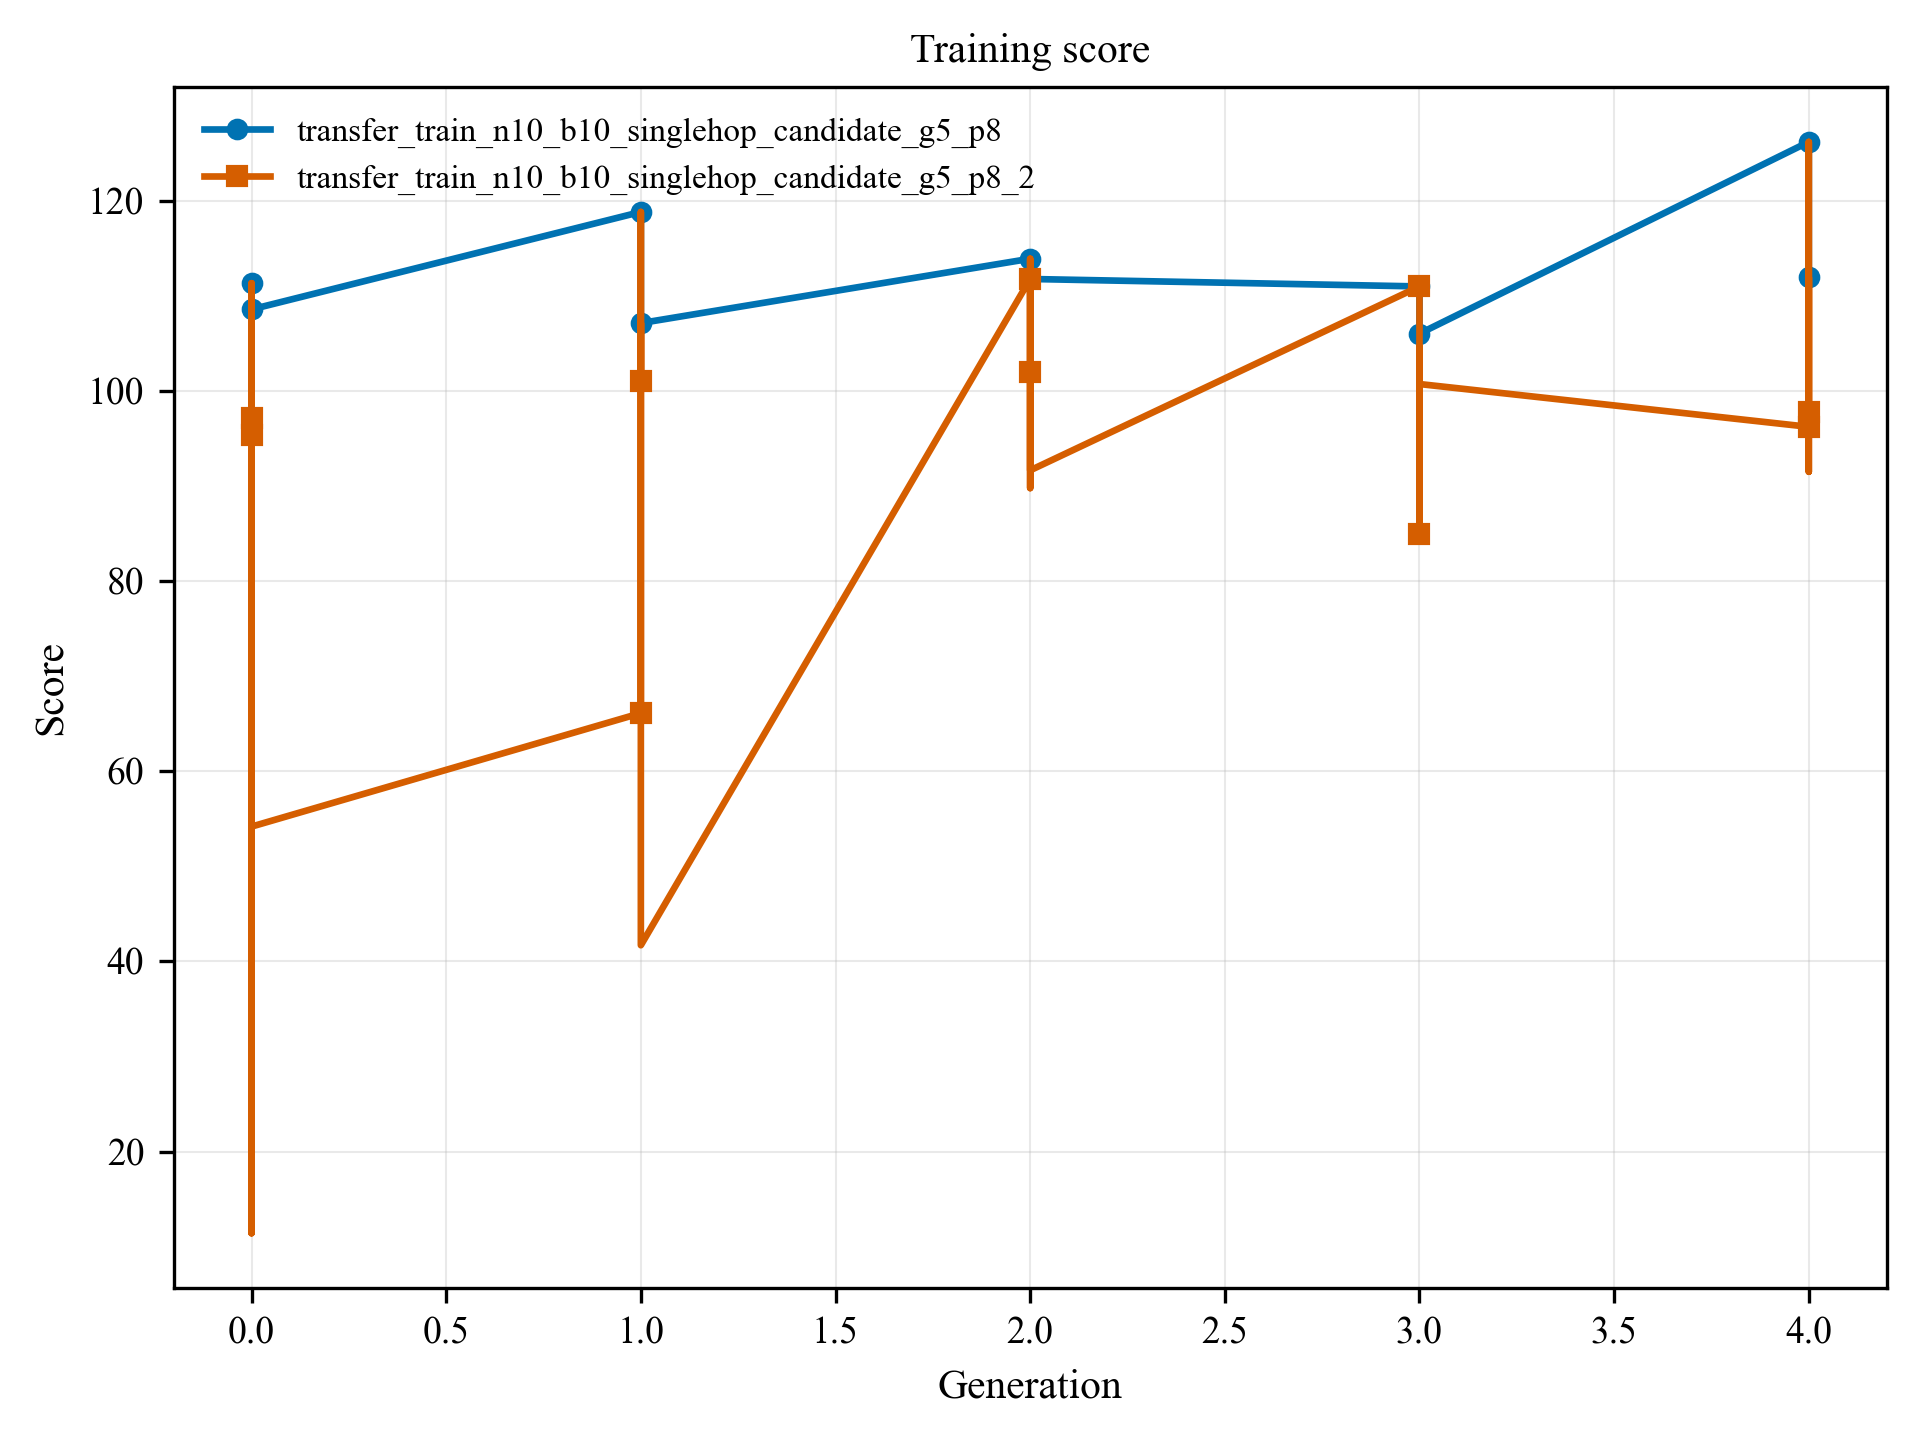
\includegraphics[width=0.48\textwidth]{../../06_analysis/paper_figures/training_round2_candidate/train_score_curve.png}
  \caption{Training-history evidence for the selected shared-parameter policy-search run. Left: reward evolution. Right: selection score evolution. These single-run curves support empirical stabilization only, not theoretical convergence.}
  \label{fig:supp_training}
\end{figure*}

Fig.~\ref{fig:supp_scale_transfer} summarizes the broad node-count and beamwidth transfer grid.
The policy is trained at $N=10$ and 10-degree beams, while the grid evaluates $N=10,20,50,100$ and 3--30 degree beams under density-preserving scaling.
The heatmap and B=10 node-count curve show the intended small-to-large transfer test; the 3-degree column remains a stress boundary.

\begin{figure*}[!t]
  \centering
  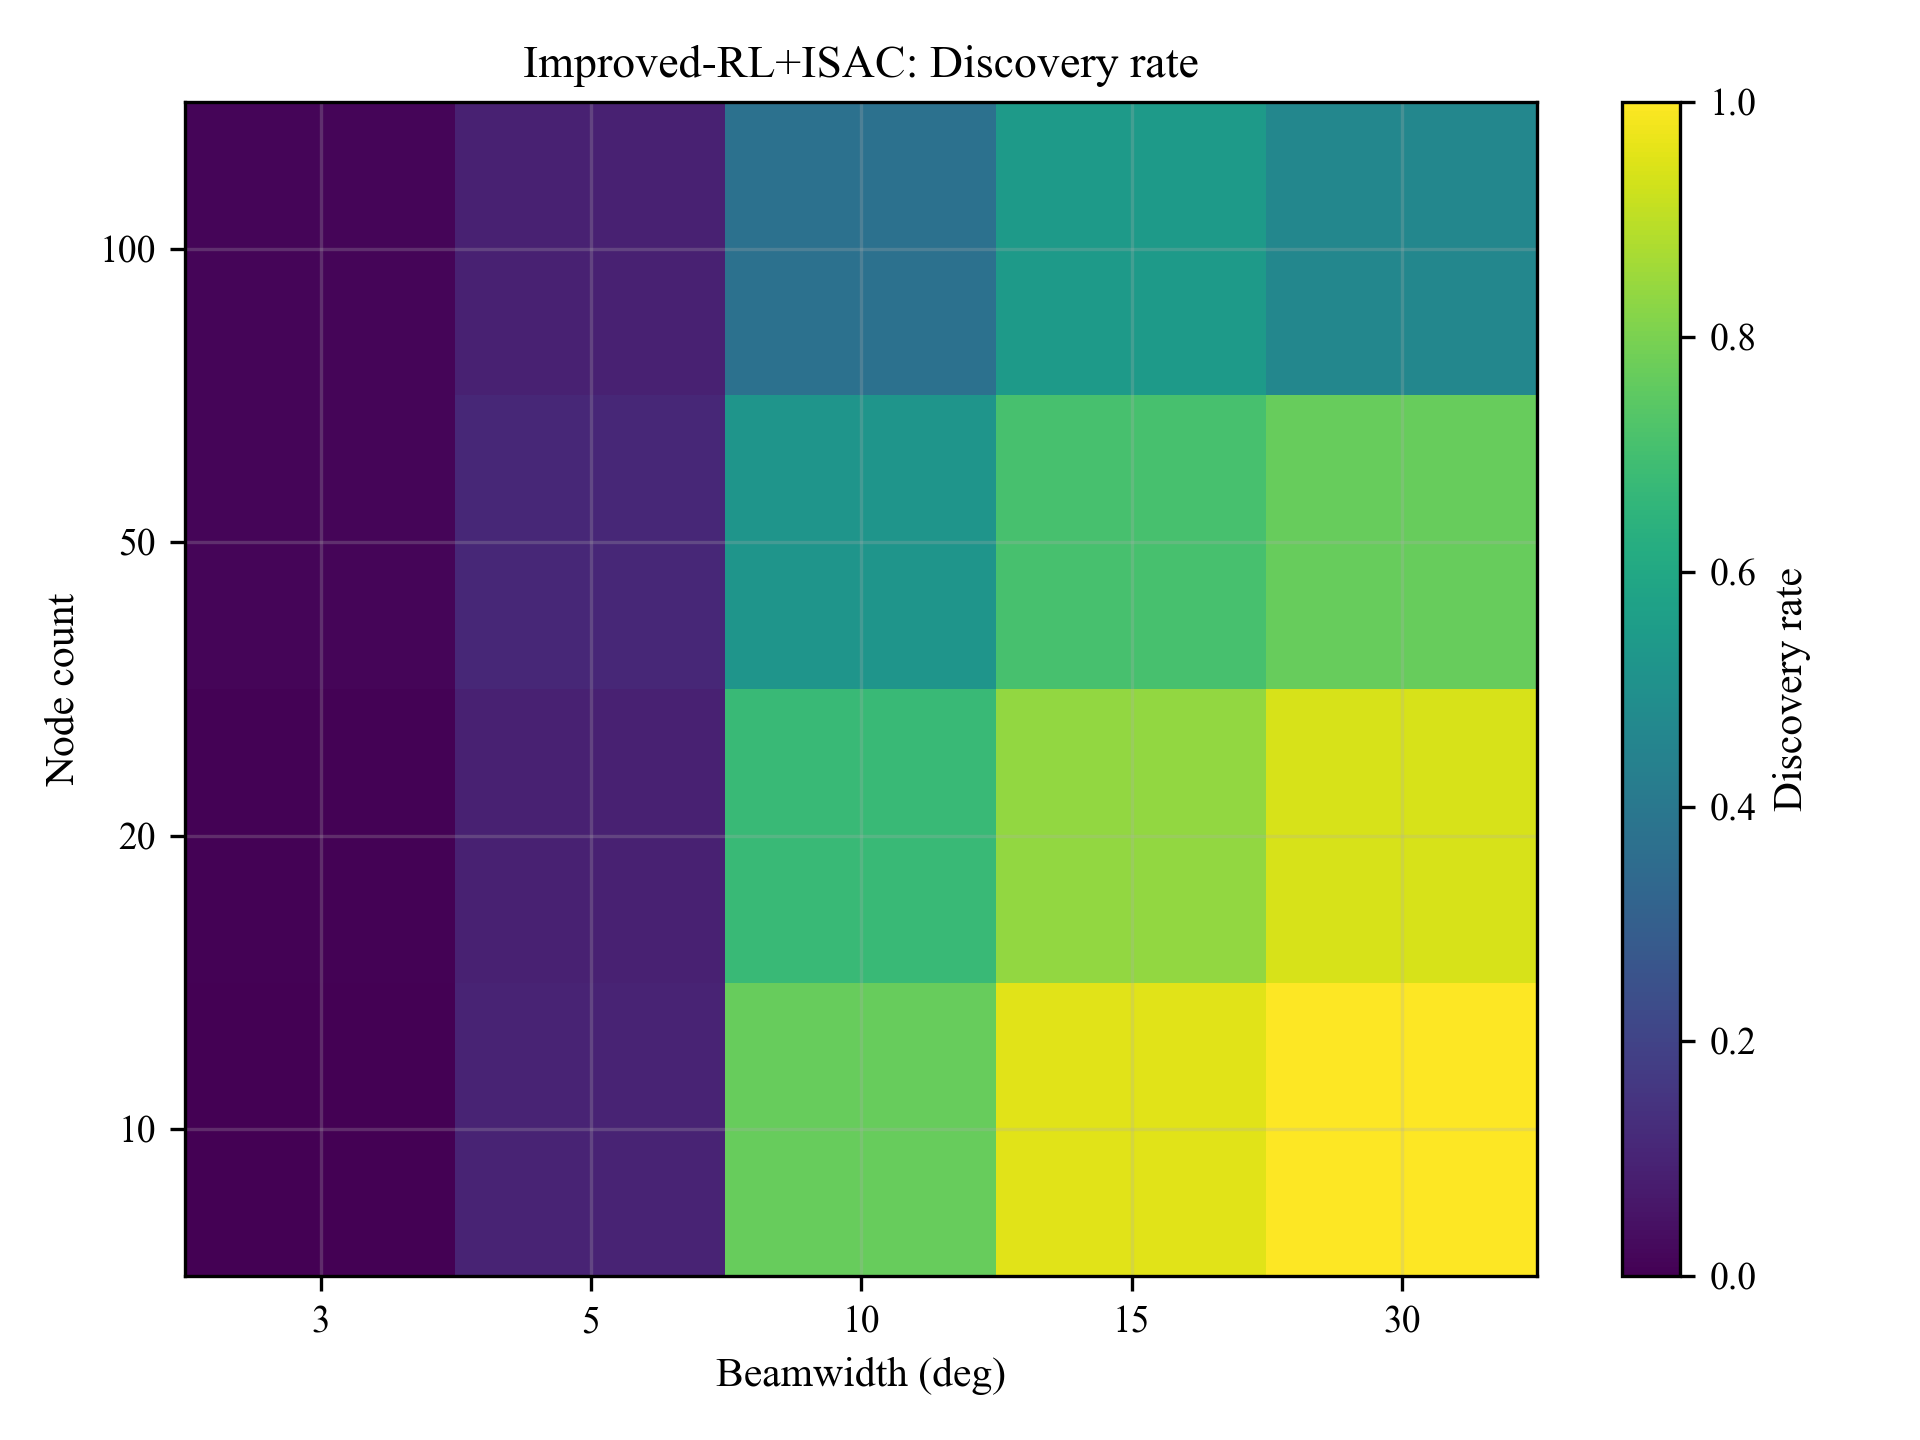
\includegraphics[width=0.48\textwidth]{../../06_analysis/paper_figures/round7_scale_beam_grid_light/density_heatmap_proposed_discovery_rate.png}
  \hfill
  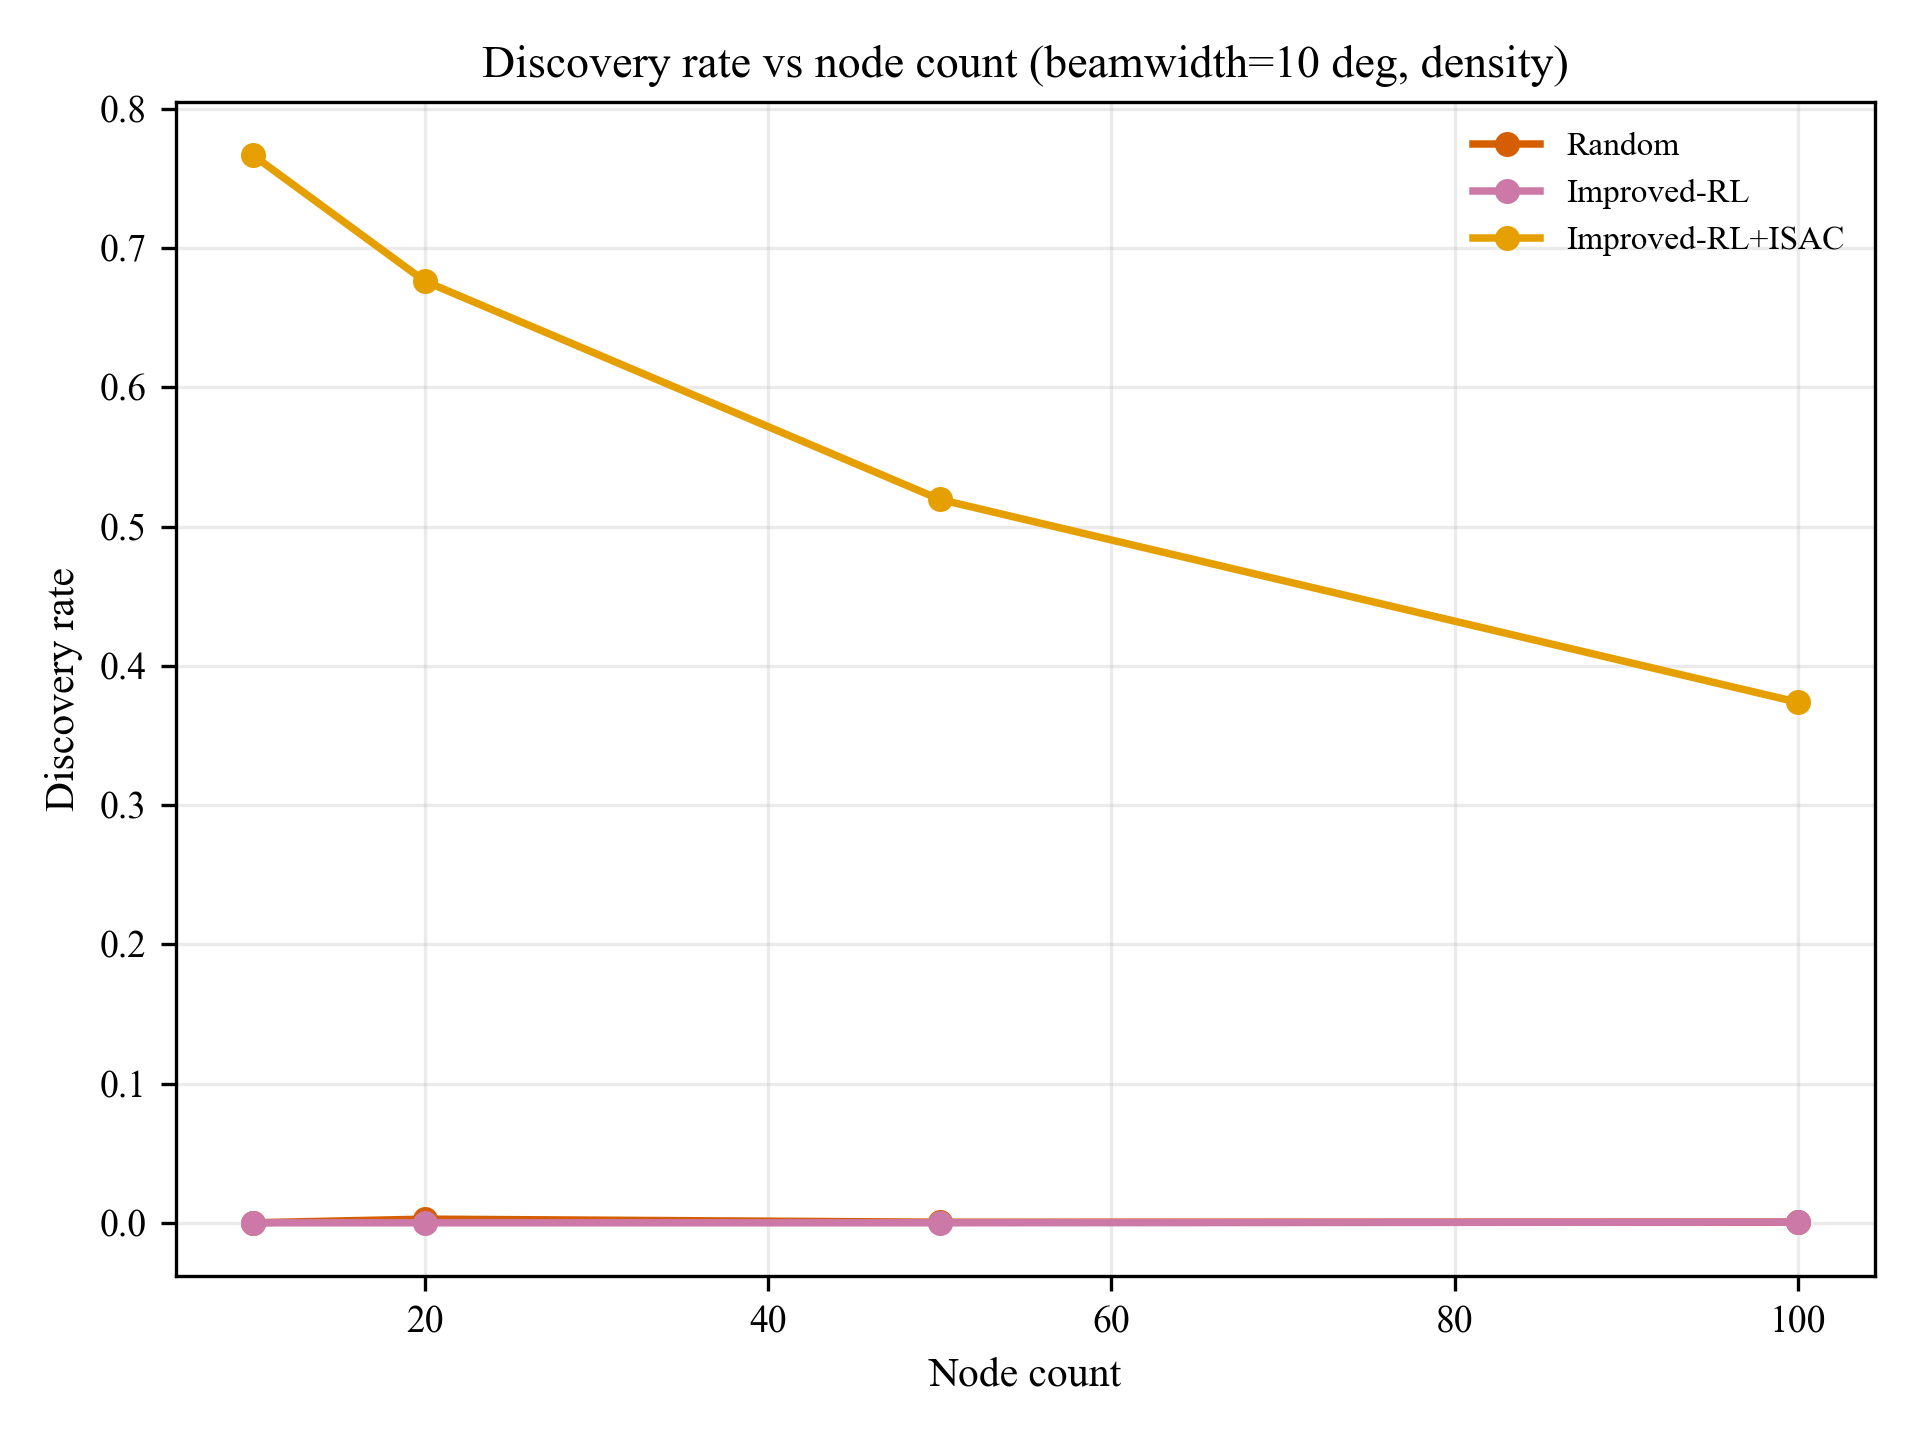
\includegraphics[width=0.48\textwidth]{../../06_analysis/paper_figures/round7_scale_beam_grid_light/density_node_count_discovery_rate_b10.png}
  \caption{Node-count and beamwidth transfer evidence. Left: proposed-policy discovery heatmap over $N=10,20,50,100$ and 3--30 degree beams. Right: B=10 node-count transfer curve.}
  \label{fig:supp_scale_transfer}
\end{figure*}

\begin{figure*}[!t]
  \centering
  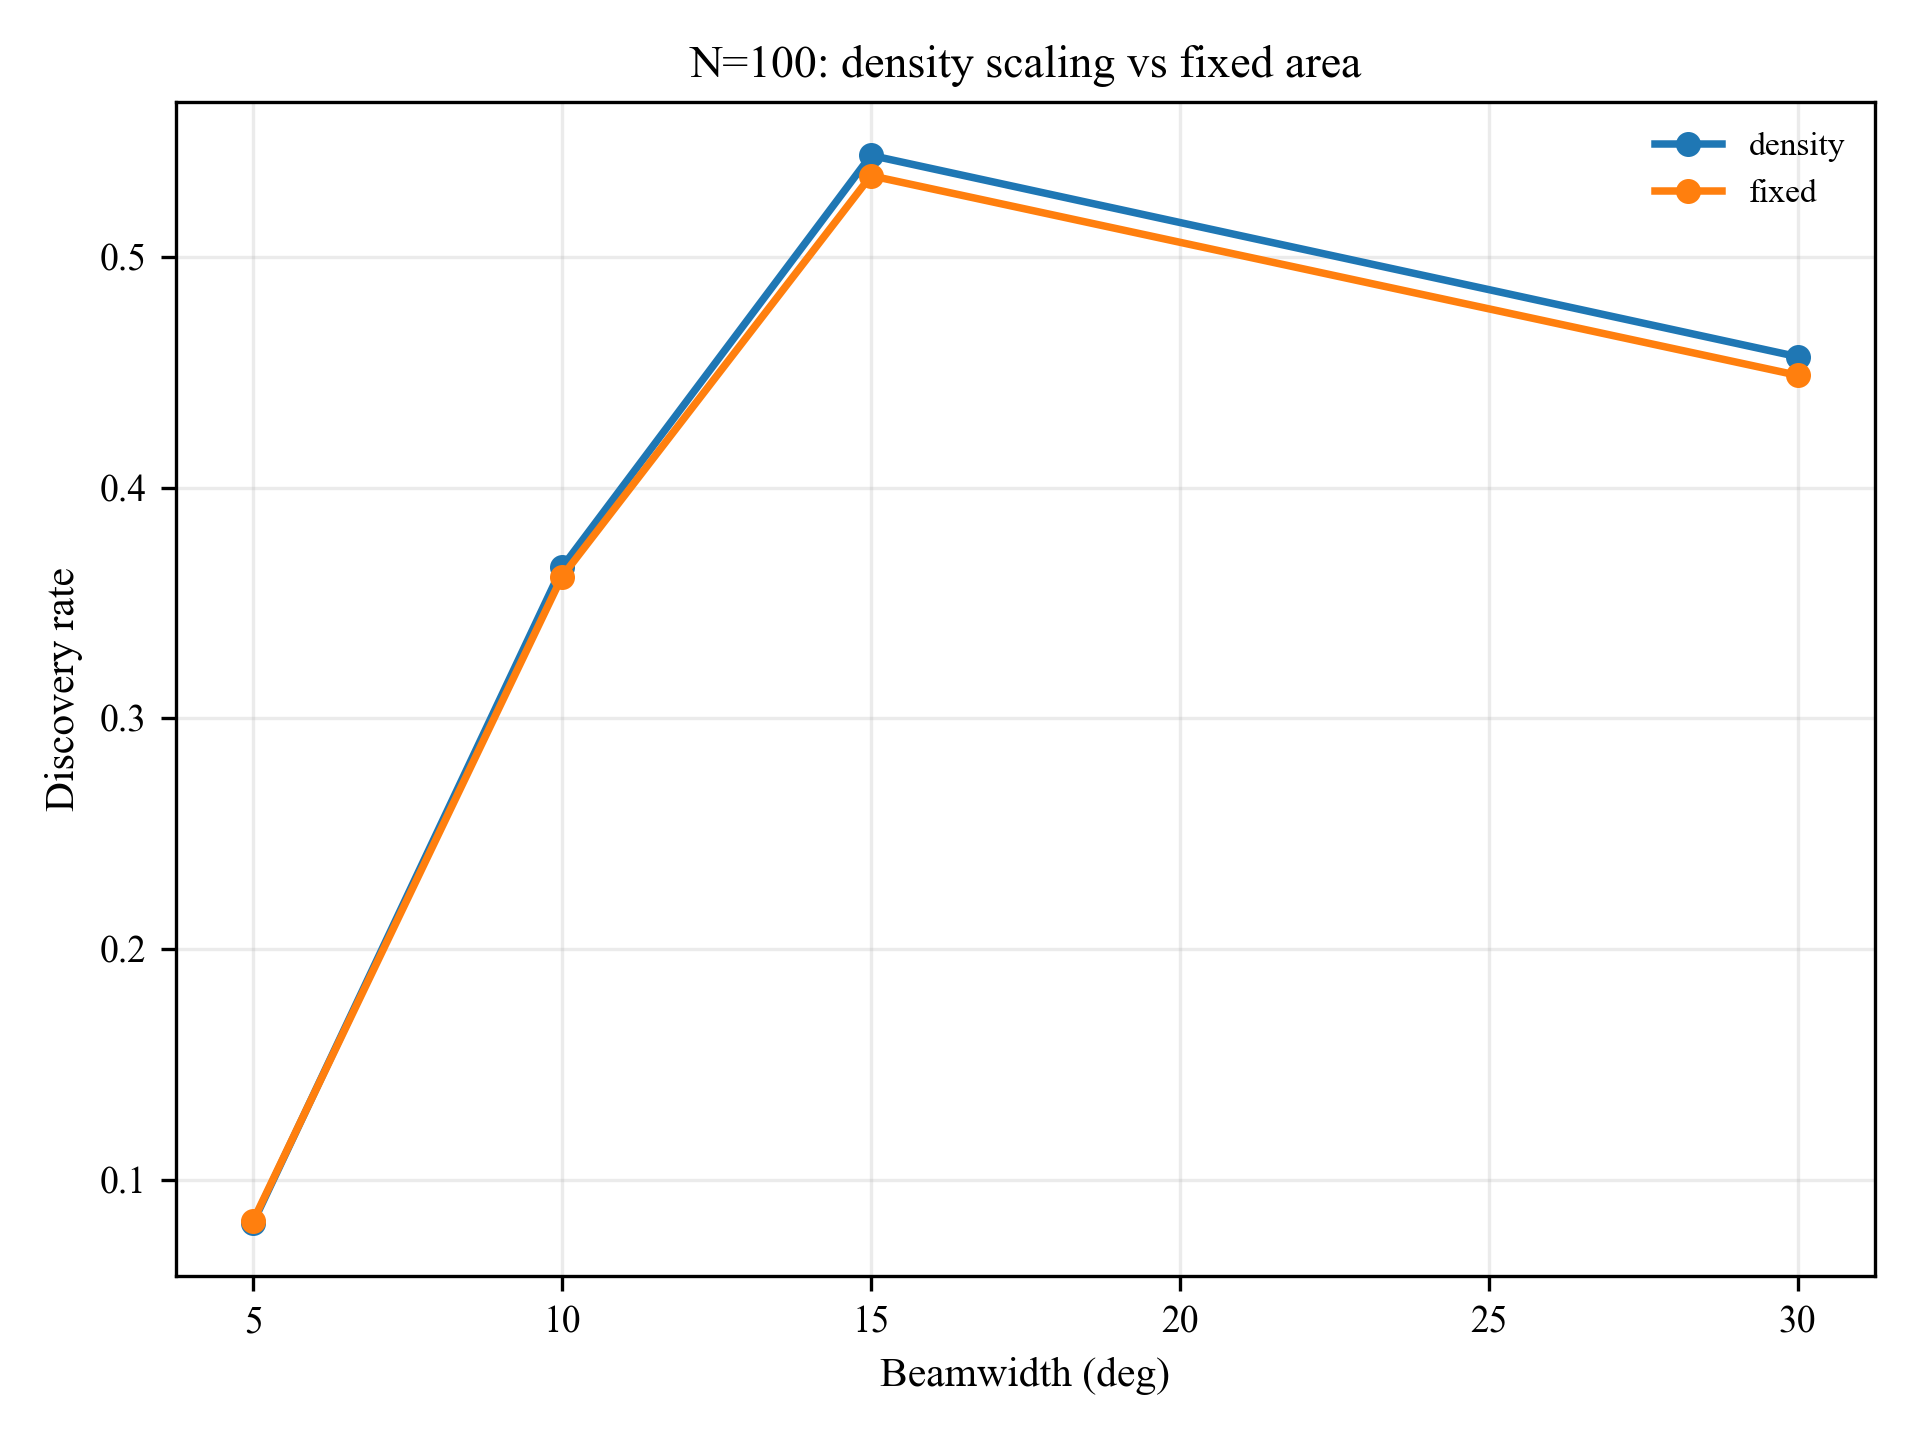
\includegraphics[width=0.48\textwidth]{../../06_analysis/paper_figures/round3_n100_transfer/area_scale_n100_discovery_rate.png}
  \hfill
  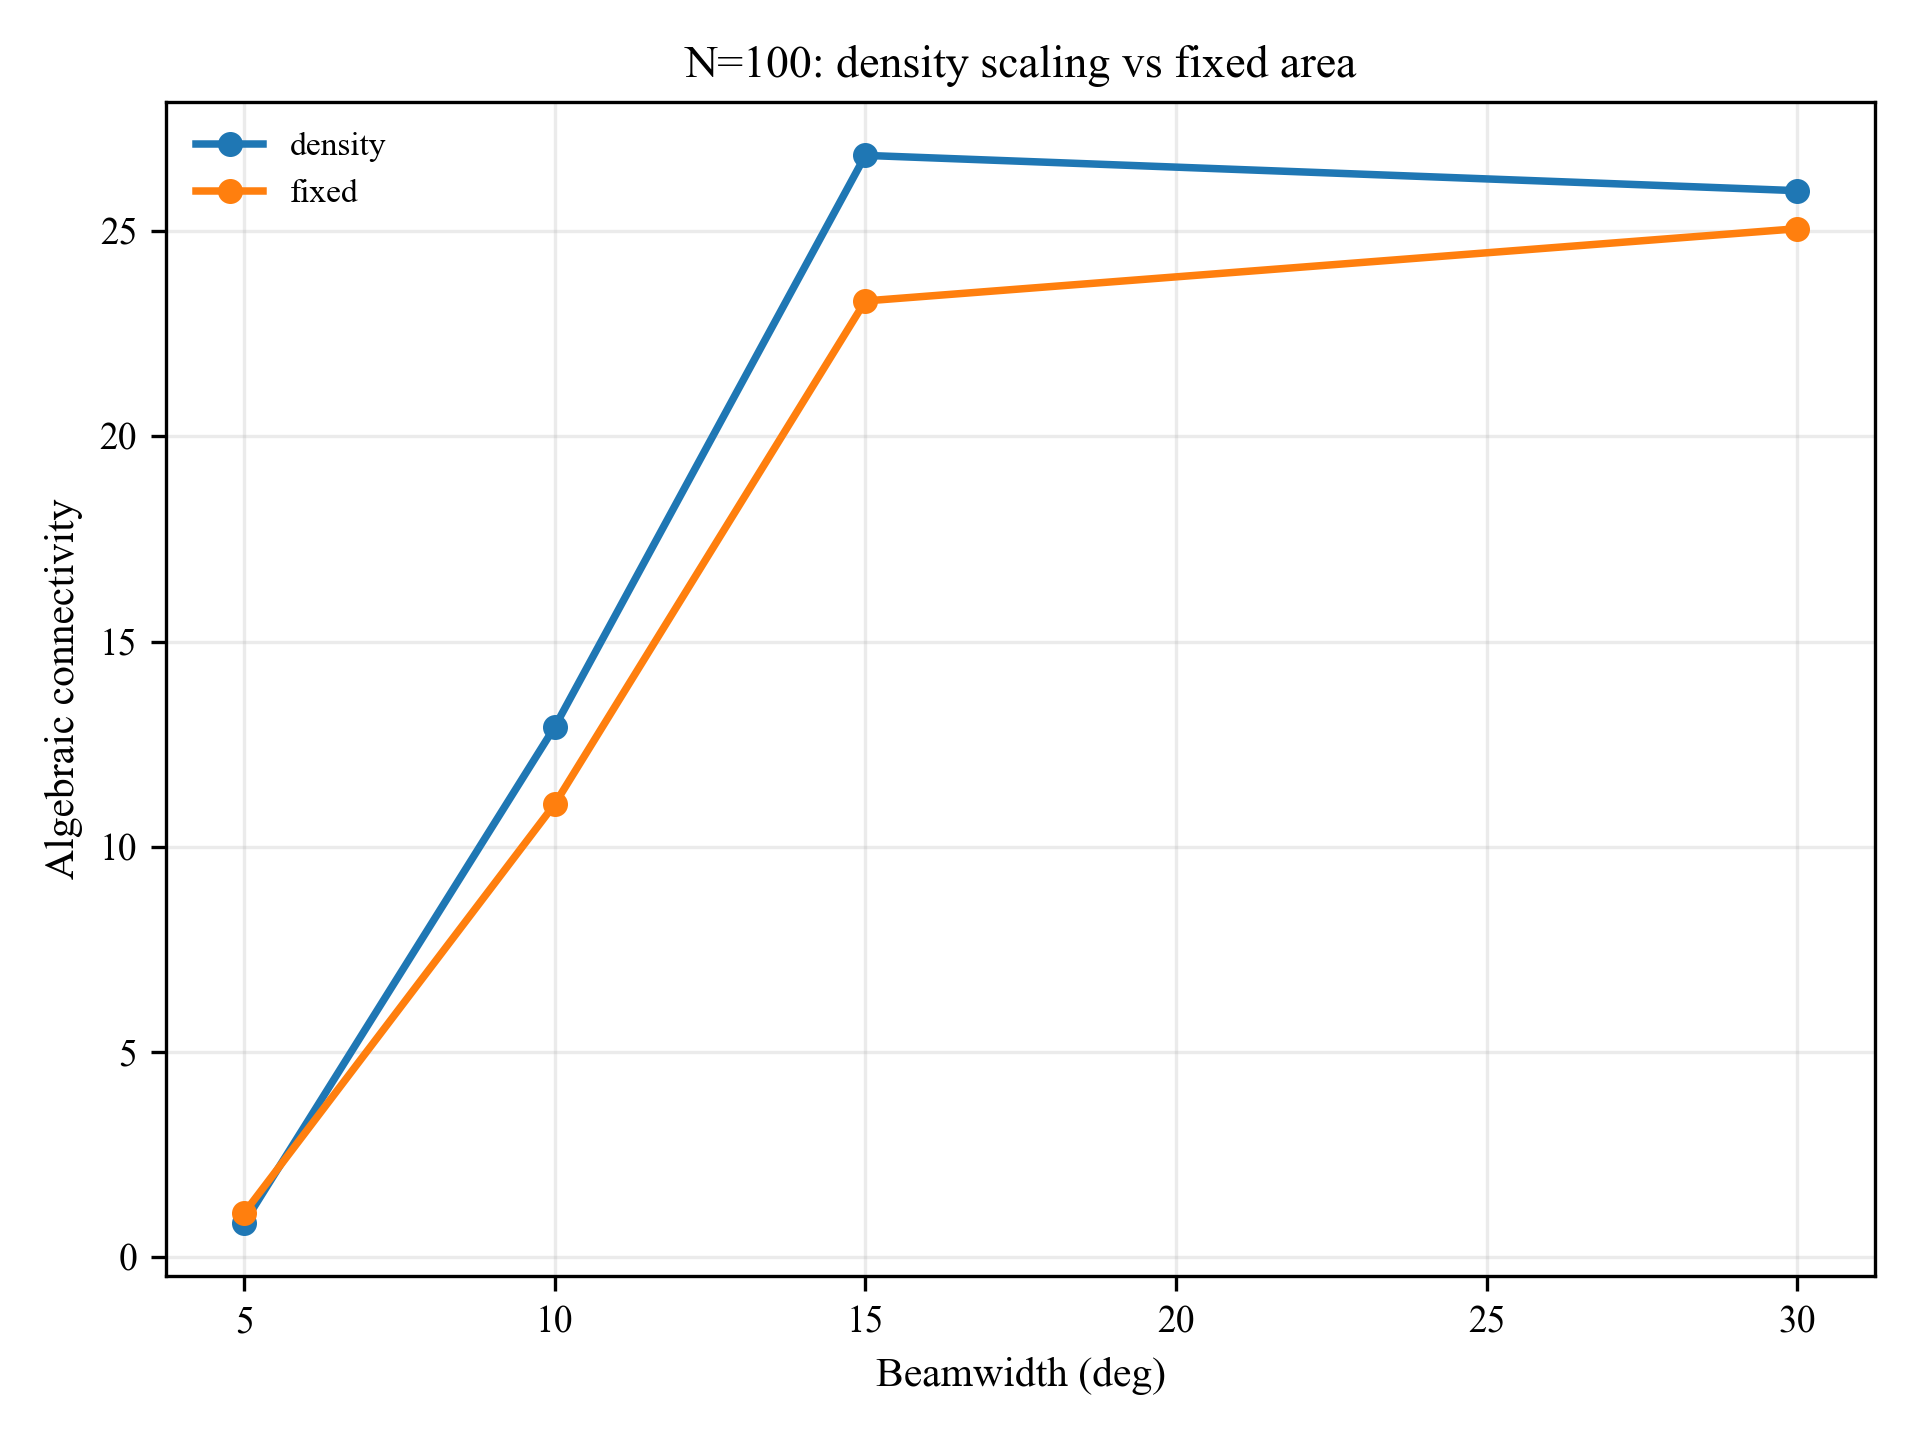
\includegraphics[width=0.48\textwidth]{../../06_analysis/paper_figures/round3_n100_transfer/area_scale_n100_lambda2.png}
  \caption{N=100 area-scaling comparison. Left: discovery rate under density-preserving and fixed-area scaling. Right: algebraic connectivity under the same scaling conventions.}
  \label{fig:supp_area_scale}
\end{figure*}

\section{Range and Time-Scale Sensitivity}

Fig.~\ref{fig:supp_range_timing} records the two implementation-sensitivity checks most directly tied to the ISAC abstraction.
The range sweep treats $\Rc$ and $\Rs$ as protocol-level support parameters; the slot-duration sweep evaluates the 5 ms slot assumption against nearby time scales under Gauss-Markov mobility.

\begin{figure*}[!t]
  \centering
  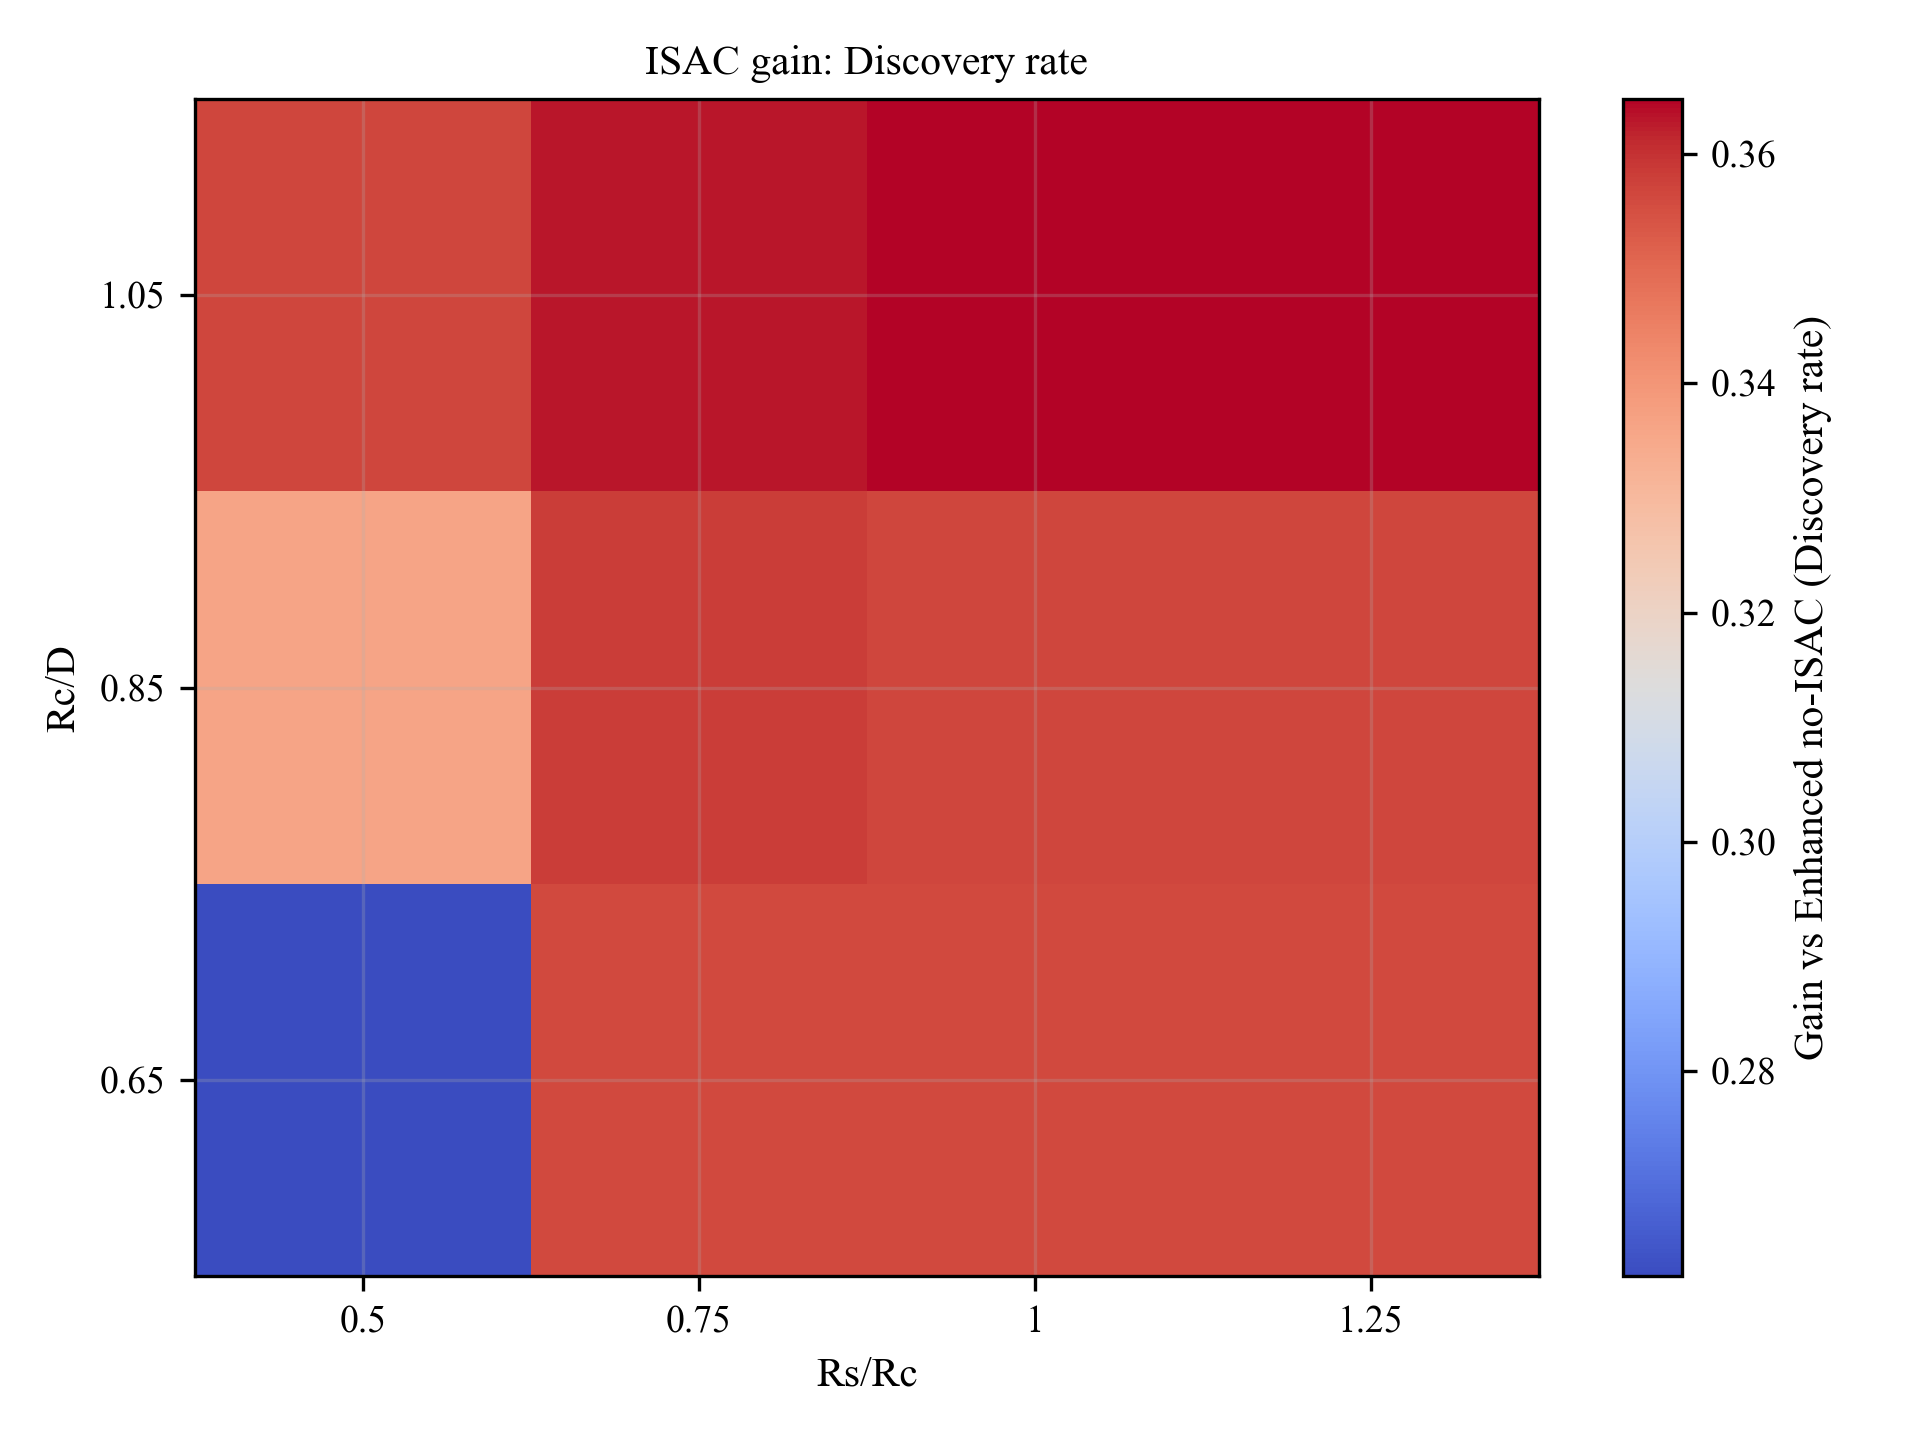
\includegraphics[width=0.48\textwidth]{../../06_analysis/paper_figures/round3_robustness/range_gain_discovery_n100_b10.png}
  \hfill
  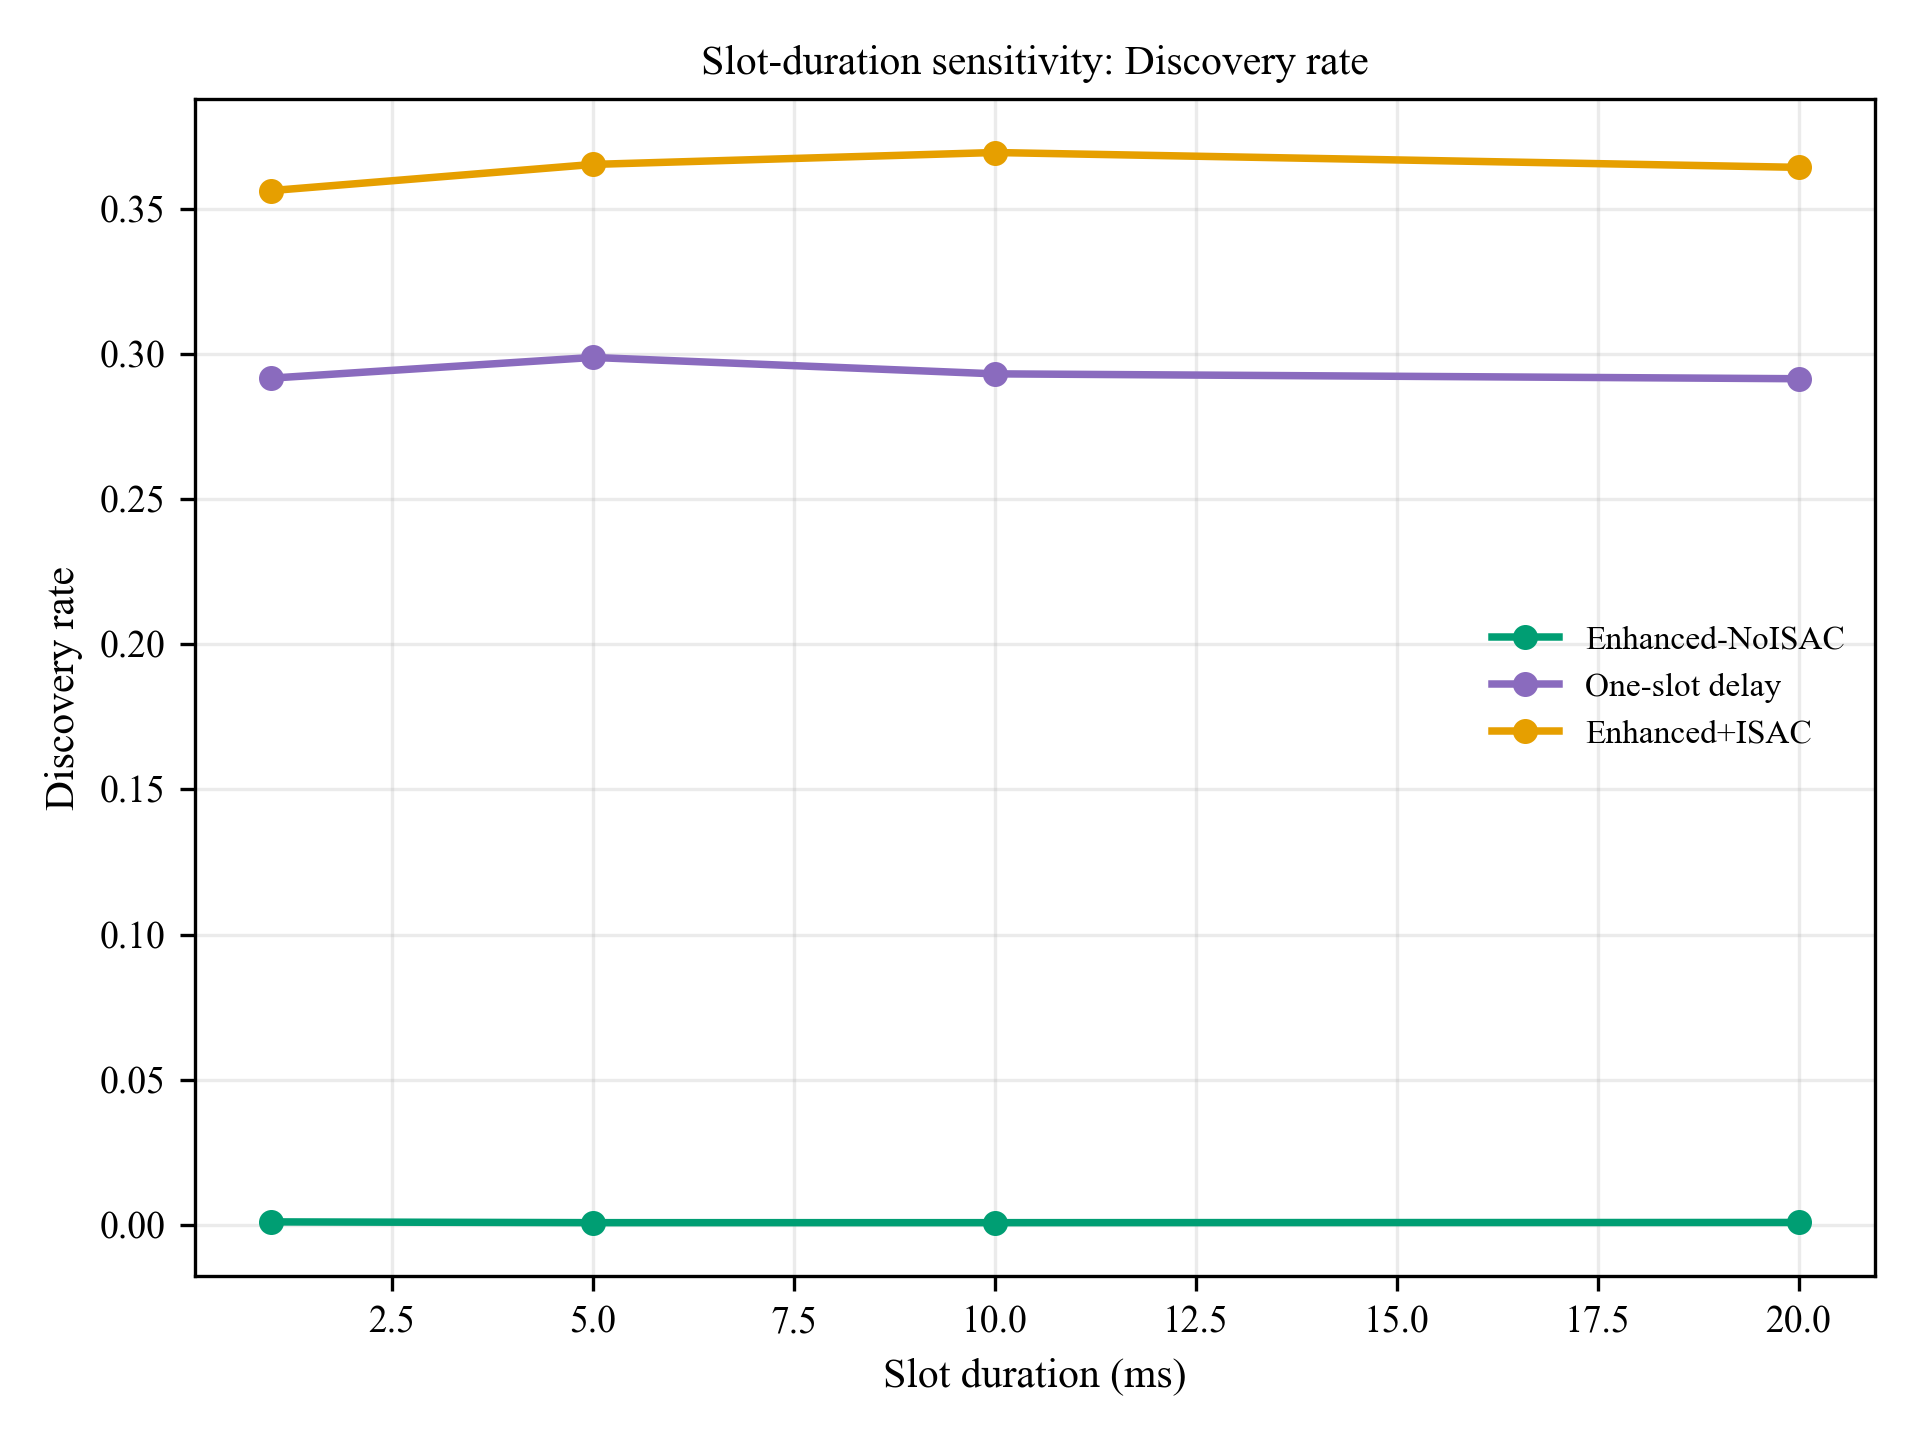
\includegraphics[width=0.48\textwidth]{../../06_analysis/paper_figures/round6_slot_duration_sensitivity/slot_duration_discovery_n100_b10.png}
  \vspace{0.4em}
  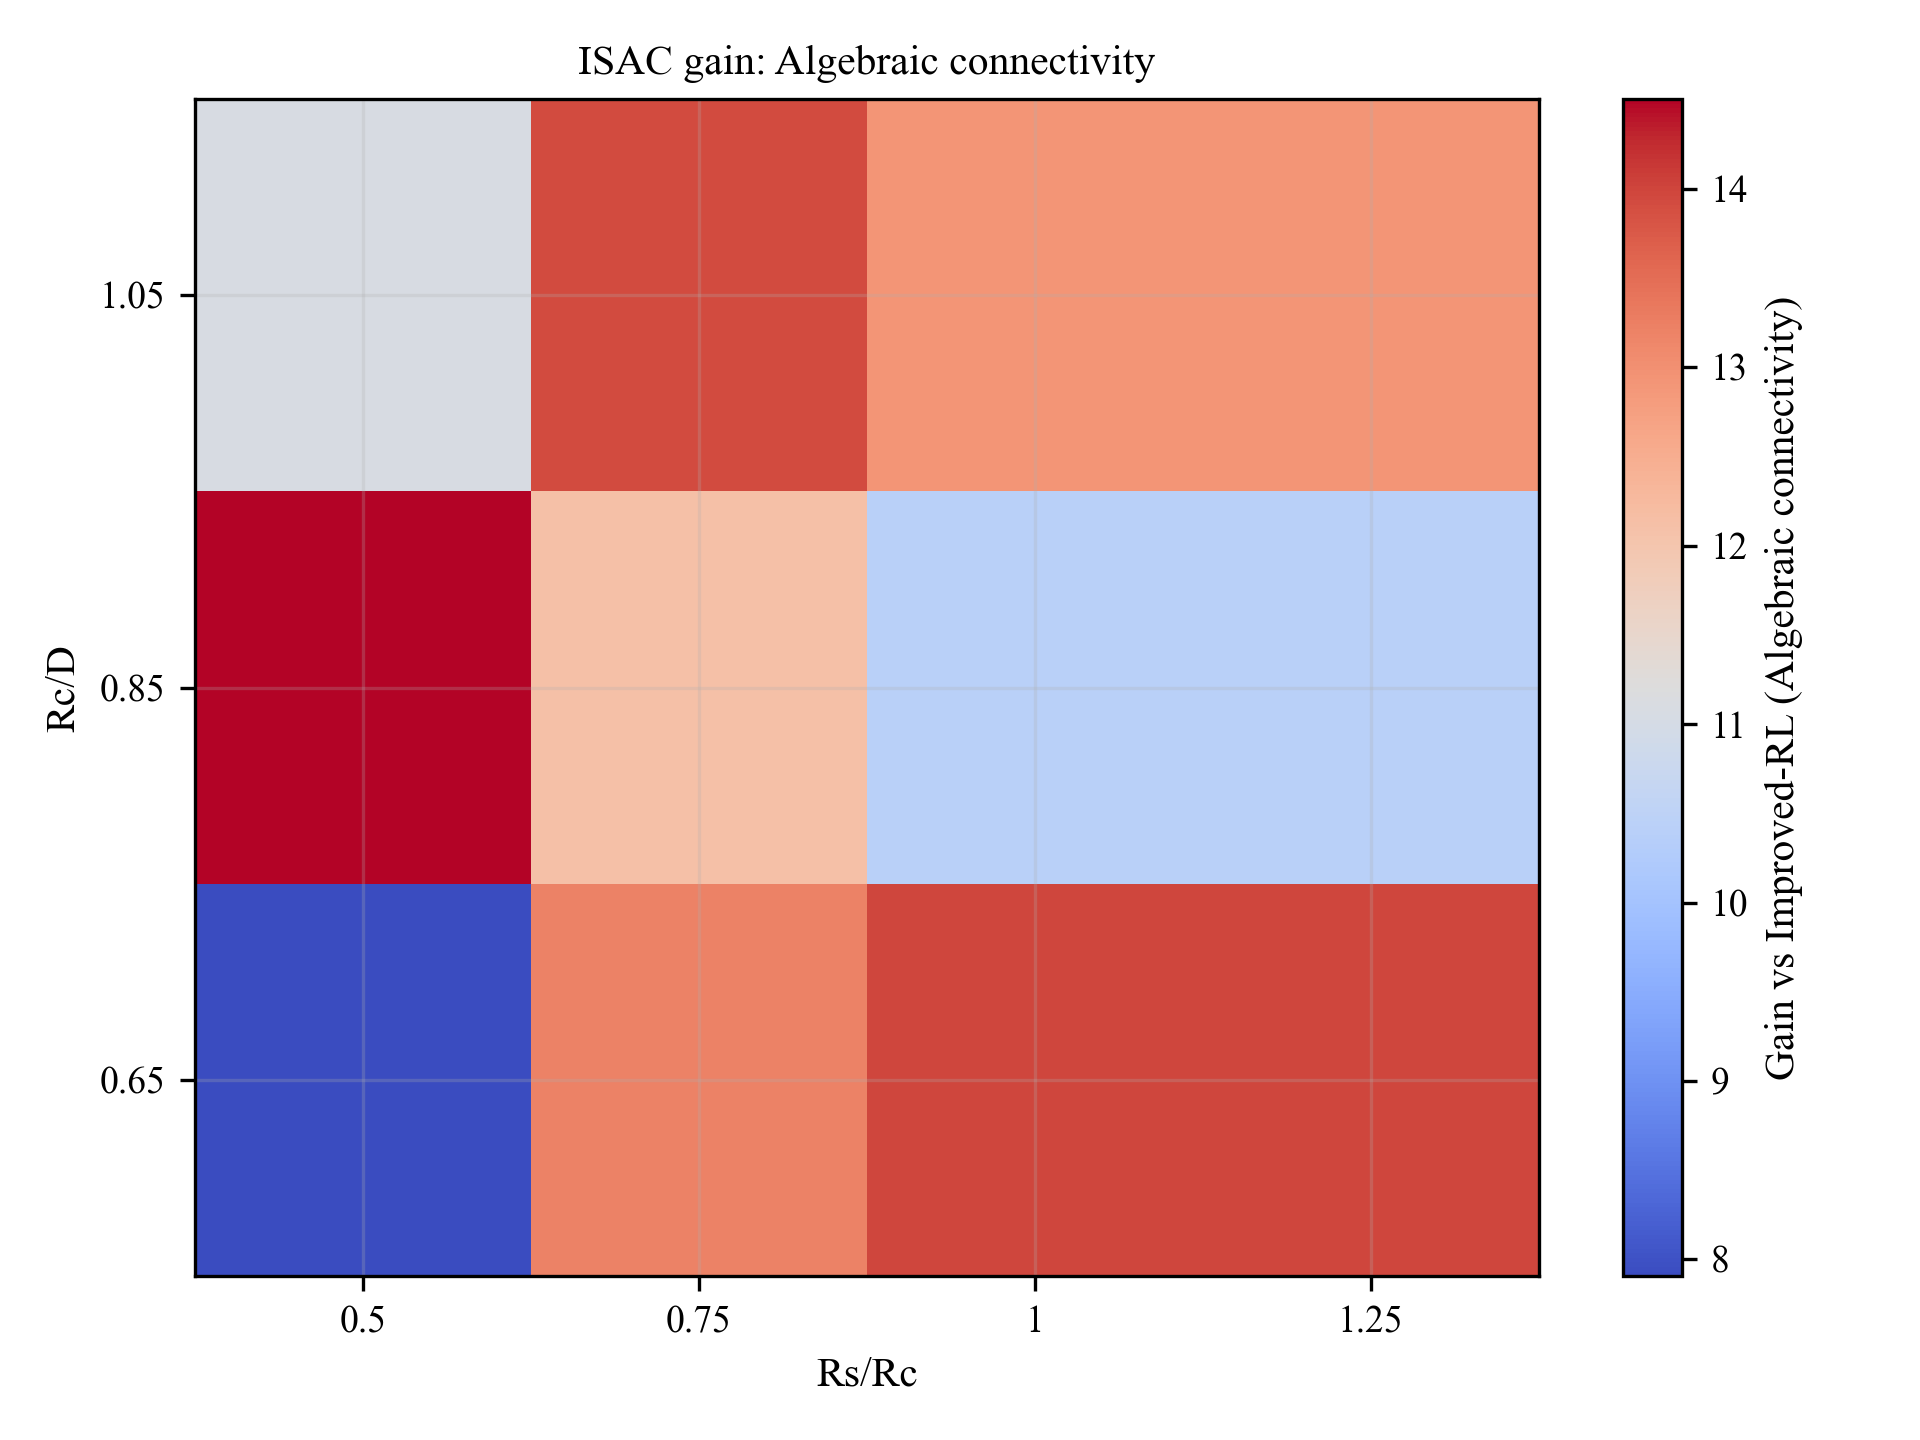
\includegraphics[width=0.48\textwidth]{../../06_analysis/paper_figures/round3_robustness/range_gain_lambda2_n100_b10.png}
  \hfill
  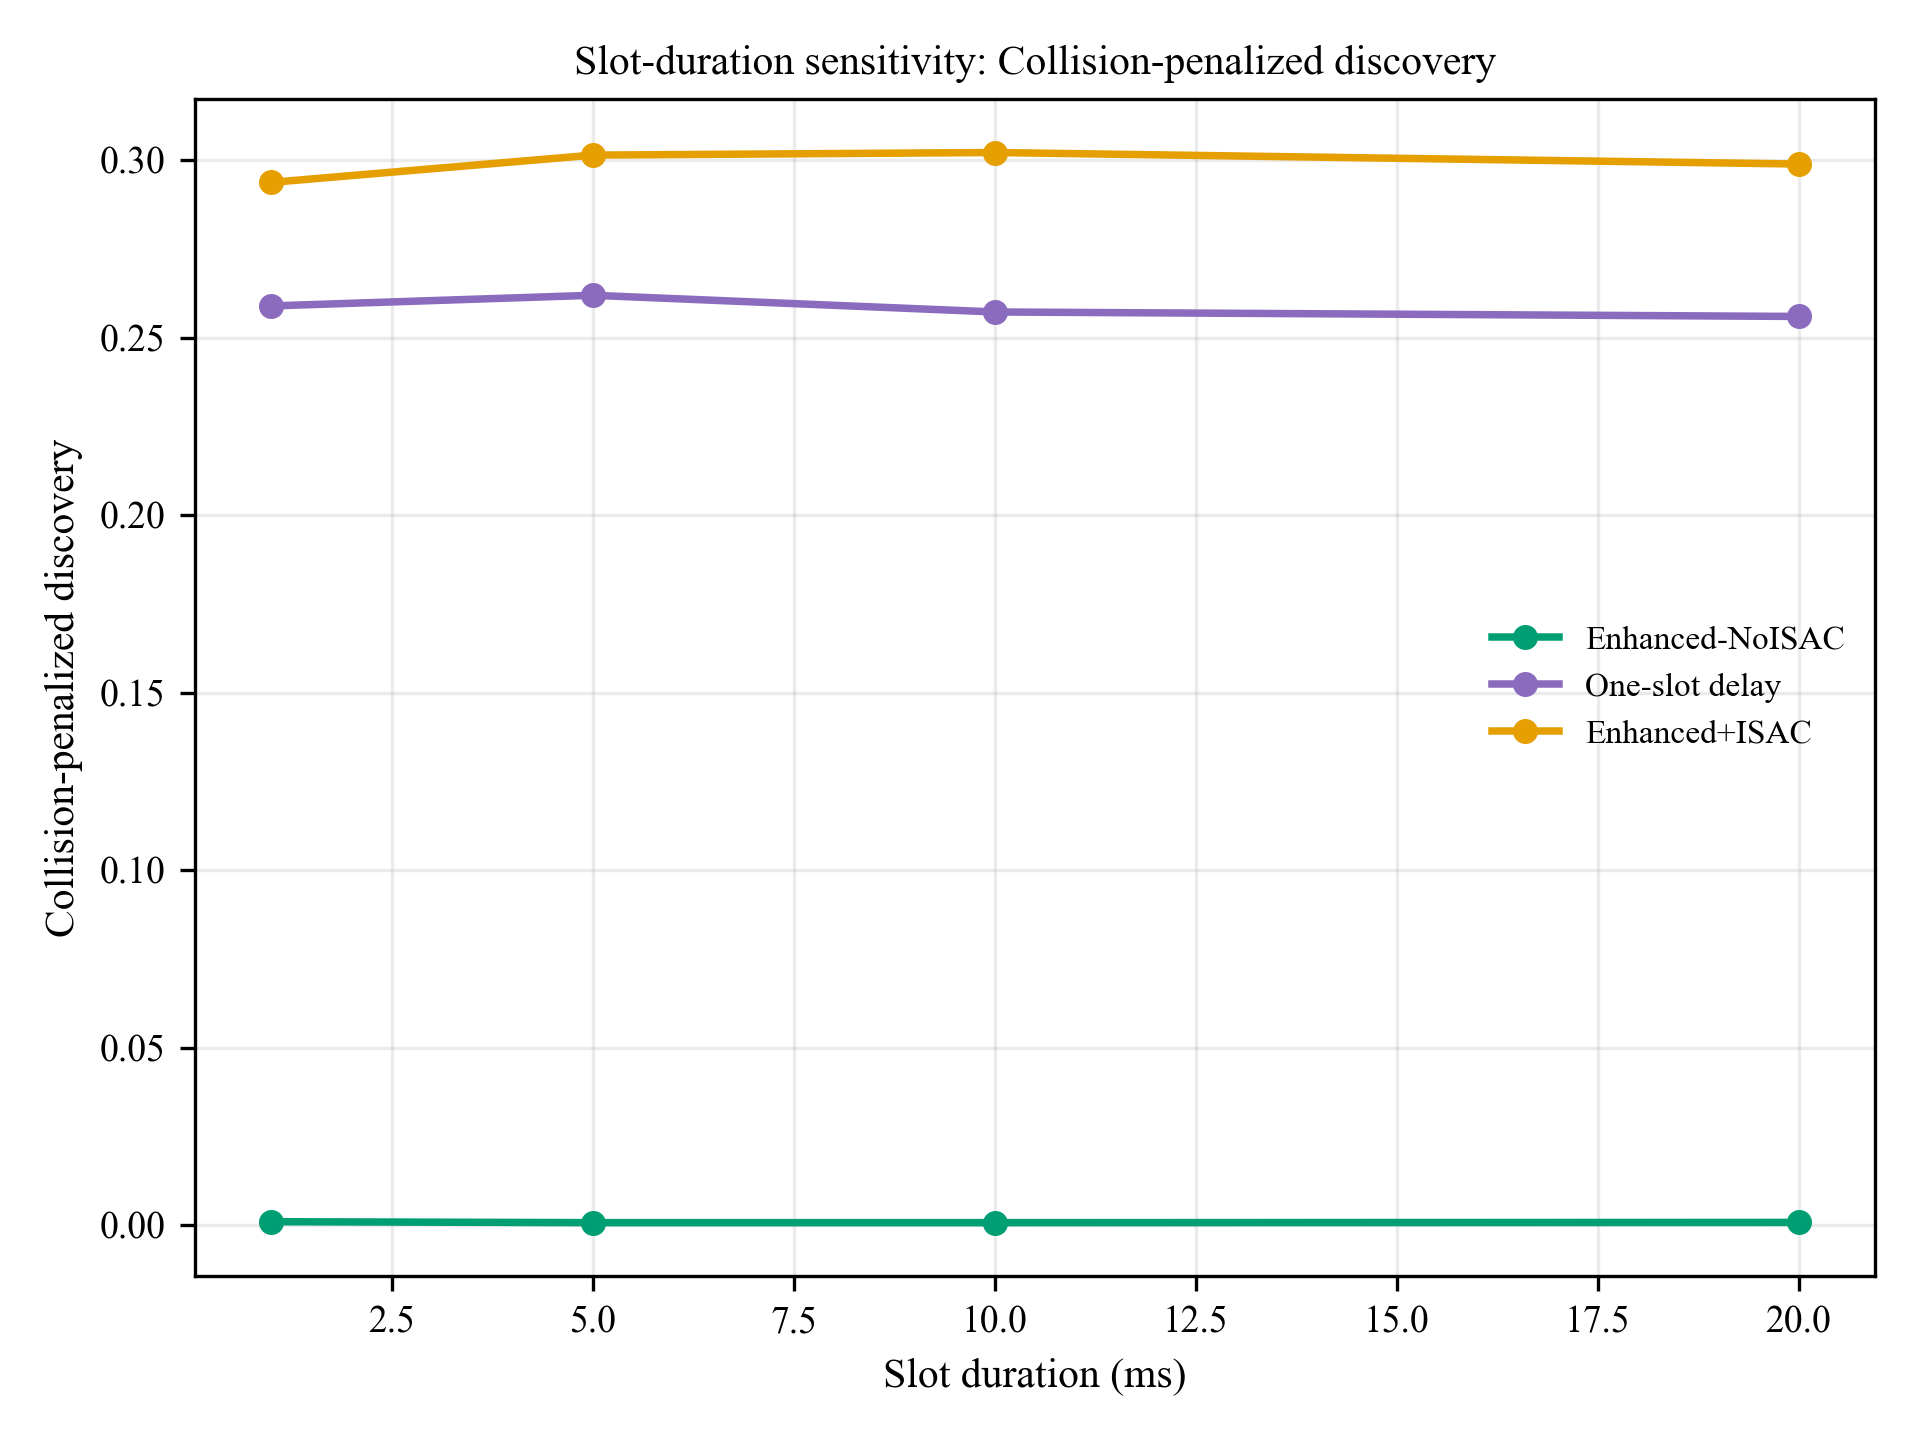
\includegraphics[width=0.48\textwidth]{../../06_analysis/paper_figures/round6_slot_duration_sensitivity/slot_duration_collision_penalized_n100_b10.png}
  \caption{Range and timing sensitivity. Top left: discovery gain over the no-ISAC counterpart as $\Rc/D$ and $\Rs/\Rc$ vary. Top right: discovery rate under slot durations from 1 ms to 20 ms. Bottom left: corresponding algebraic-connectivity gain. Bottom right: collision-penalized discovery under slot-duration variation.}
  \label{fig:supp_range_timing}
\end{figure*}

\section{Beamwidth Stress}

The main paper reports 5--30 degree transfer values in the compact N=100 table.
Fig.~\ref{fig:supp_beam_stress} shows the broader N=100 stress sweep including 3 degrees.
The 3-degree case is intentionally treated as a failure-boundary regime.

\begin{figure*}[!t]
  \centering
  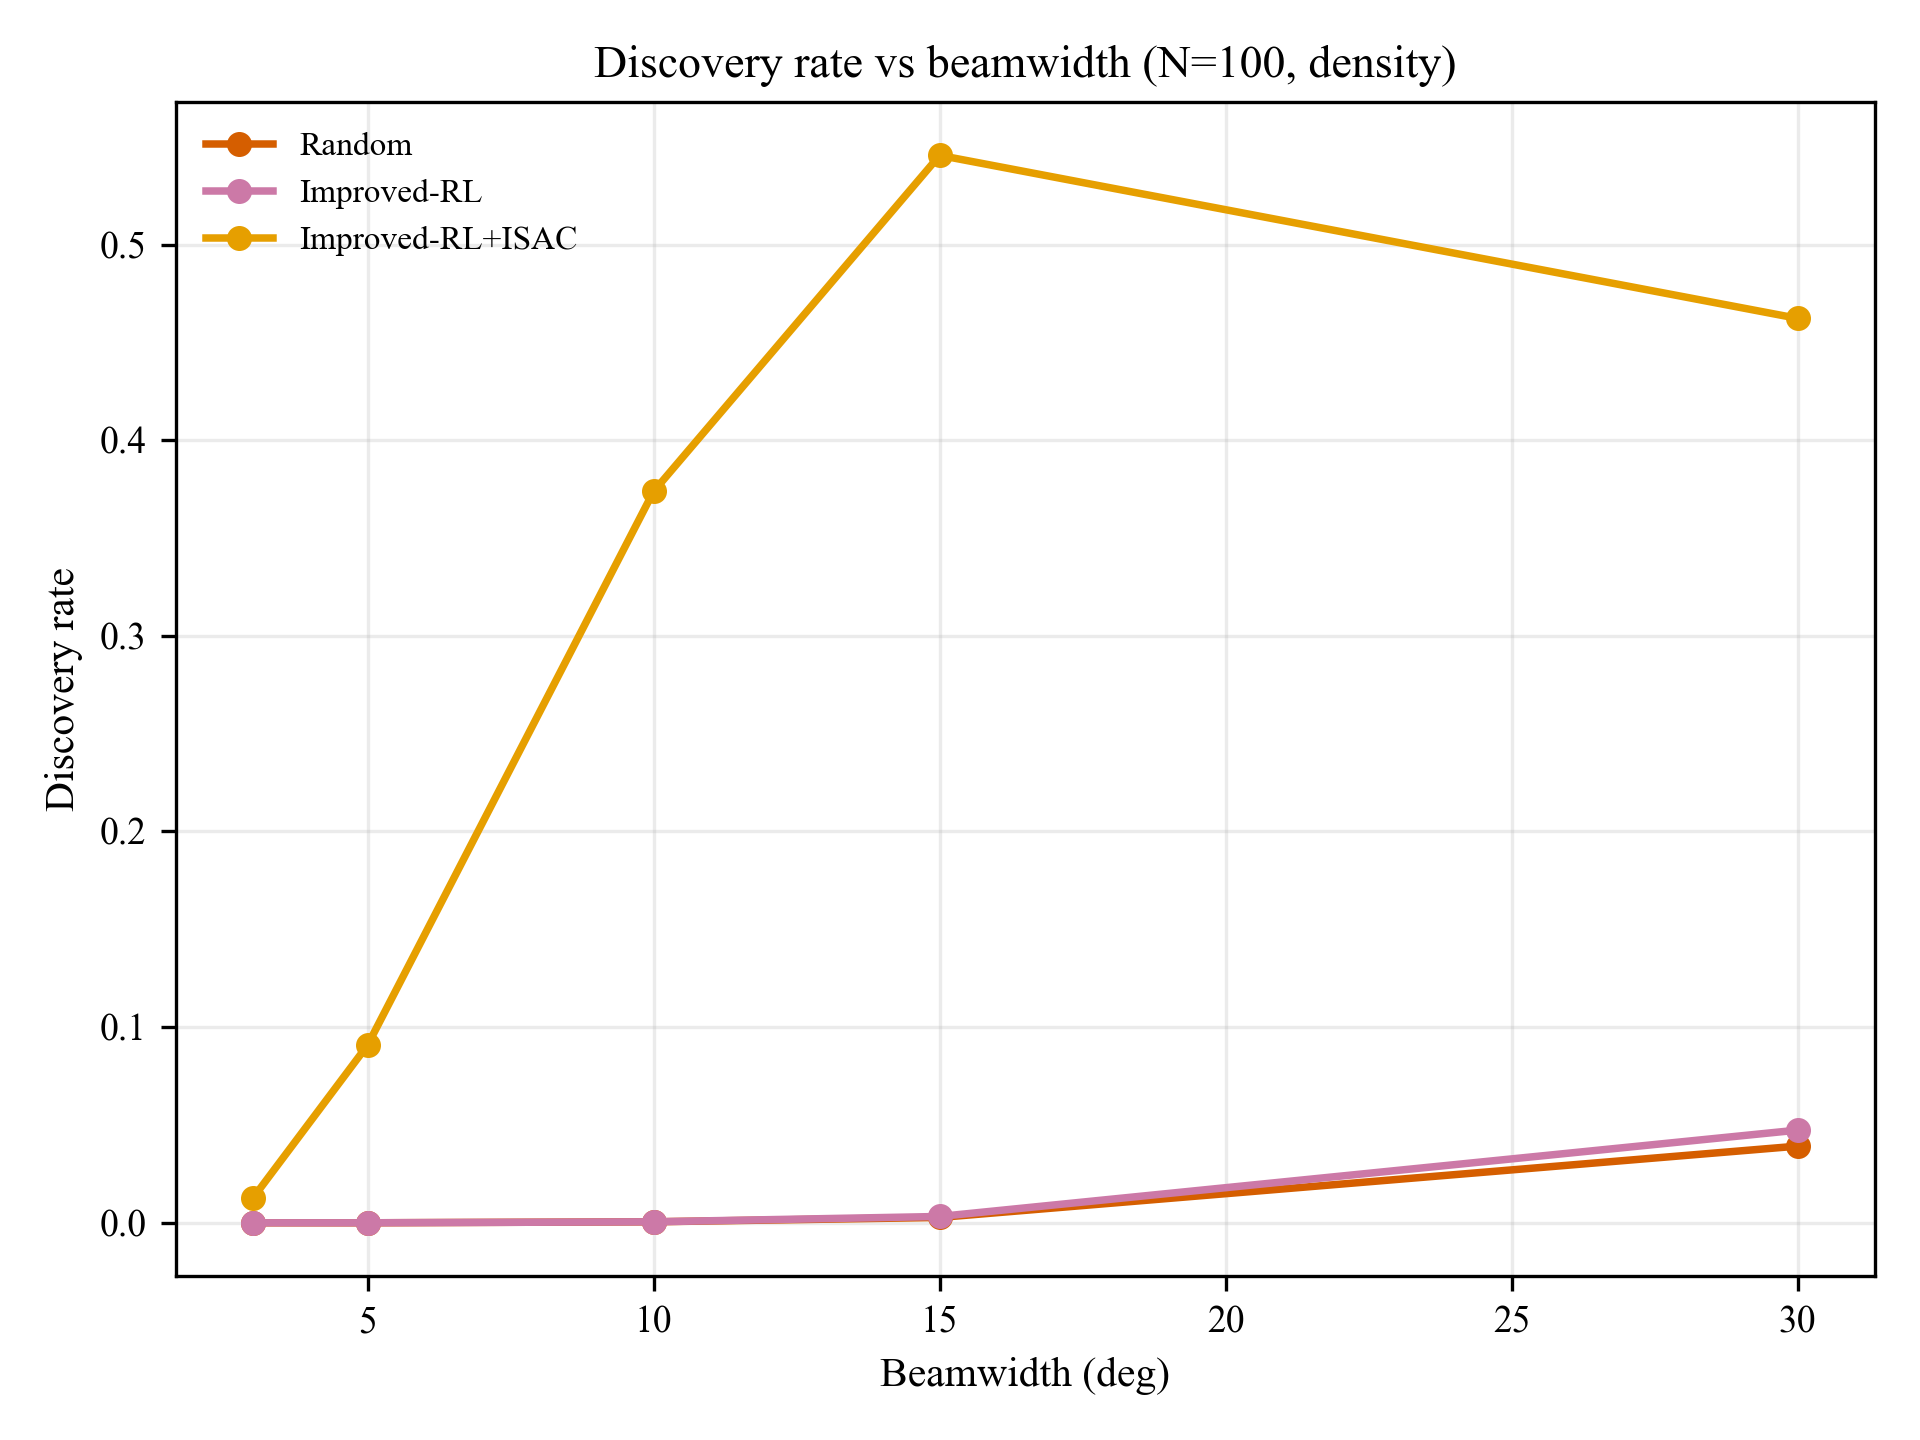
\includegraphics[width=0.32\textwidth]{../../06_analysis/paper_figures/round7_scale_beam_grid_light/density_beamwidth_discovery_rate_n100.png}
  \hfill
  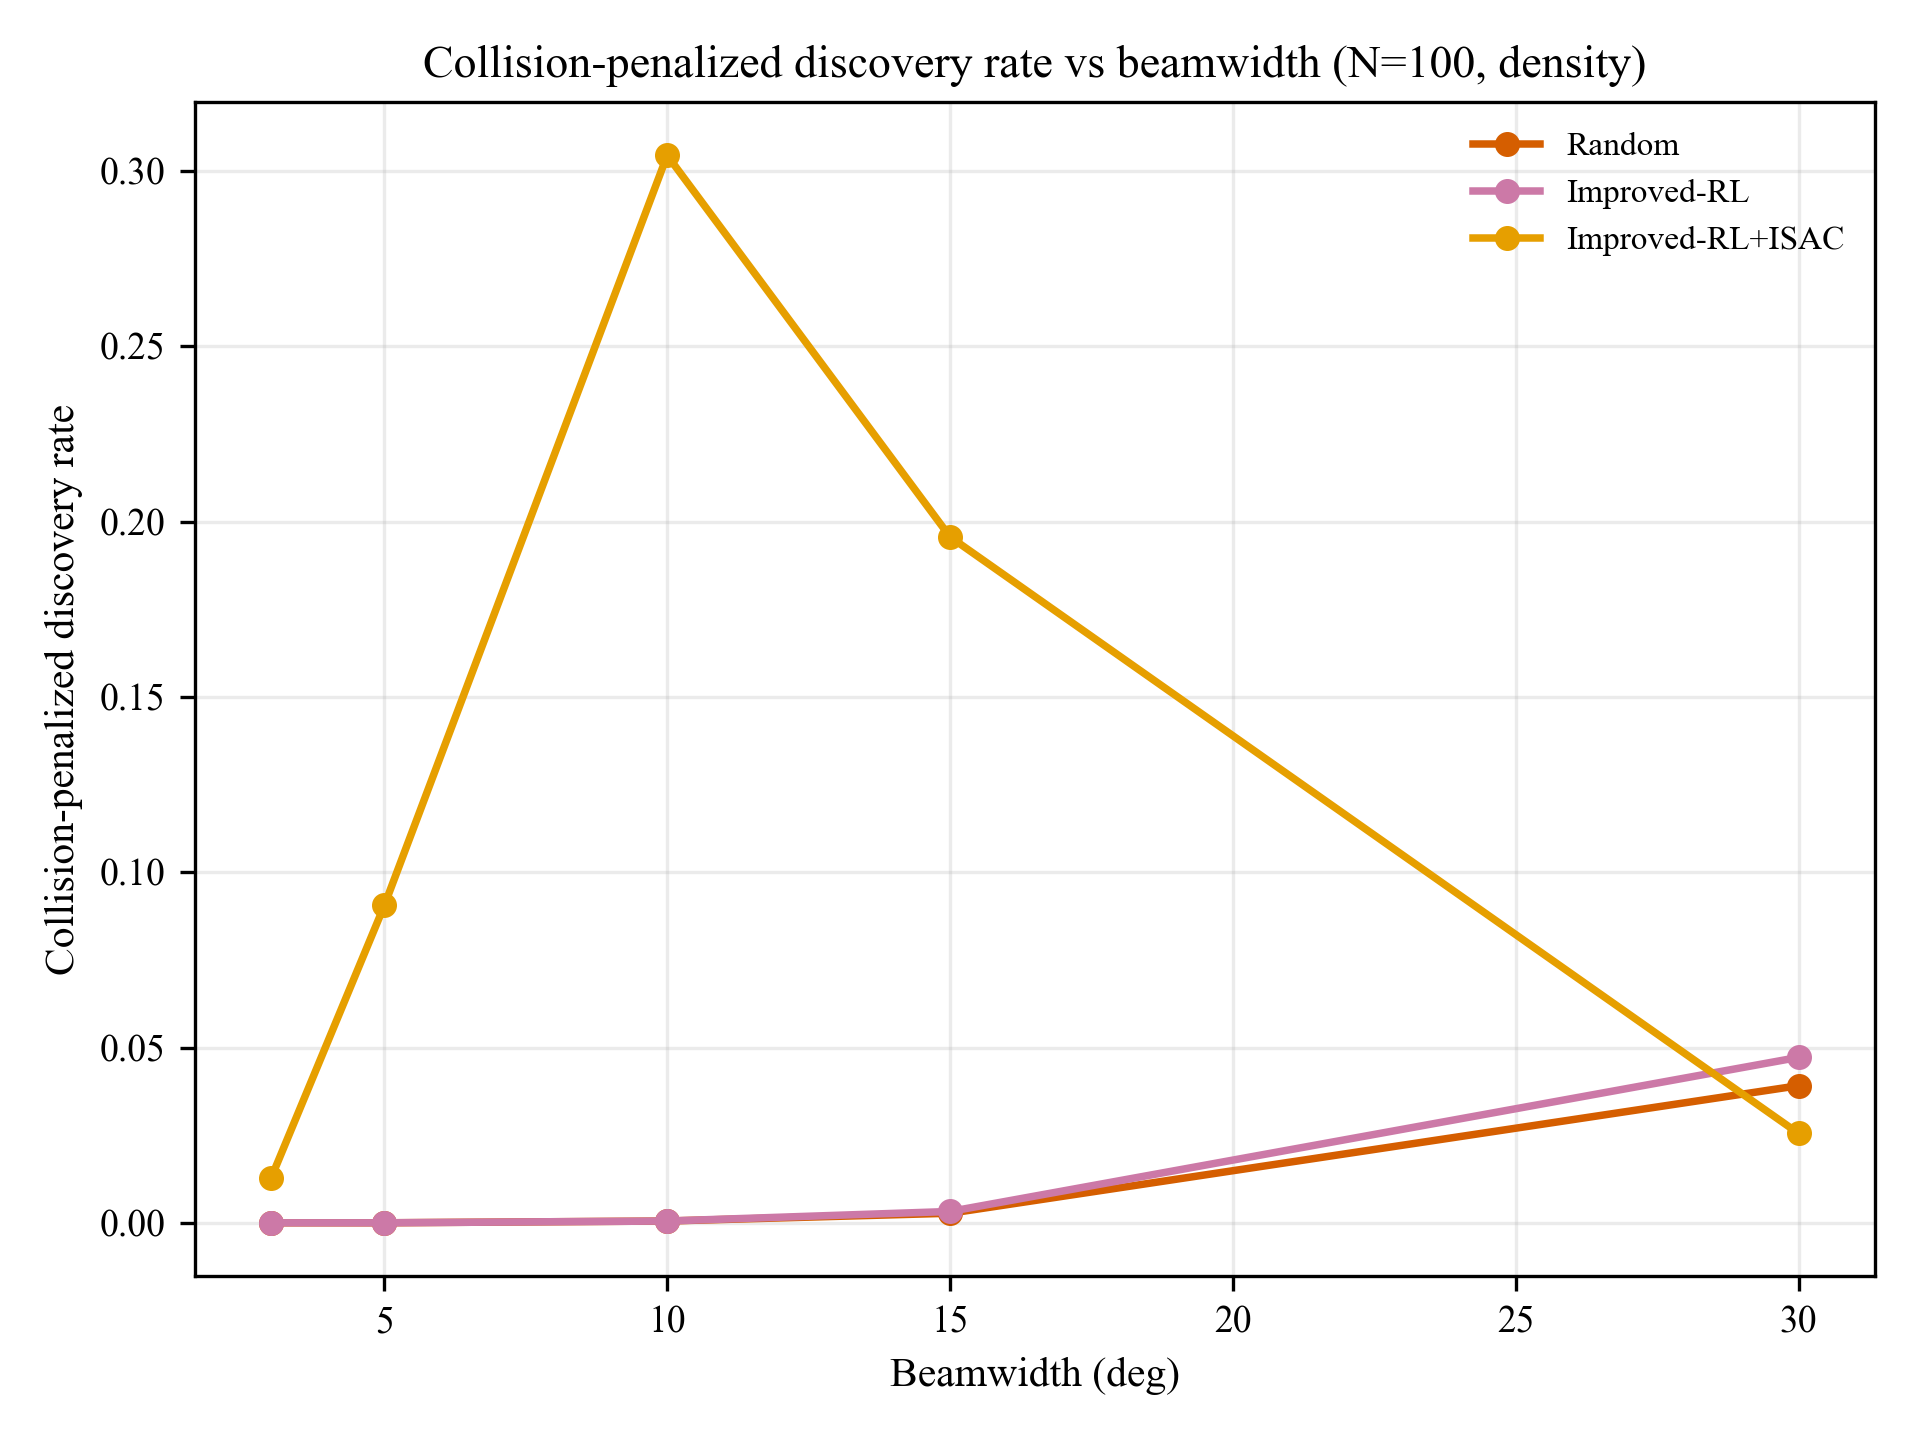
\includegraphics[width=0.32\textwidth]{../../06_analysis/paper_figures/round7_scale_beam_grid_light/density_beamwidth_collision_penalized_discovery_n100.png}
  \hfill
  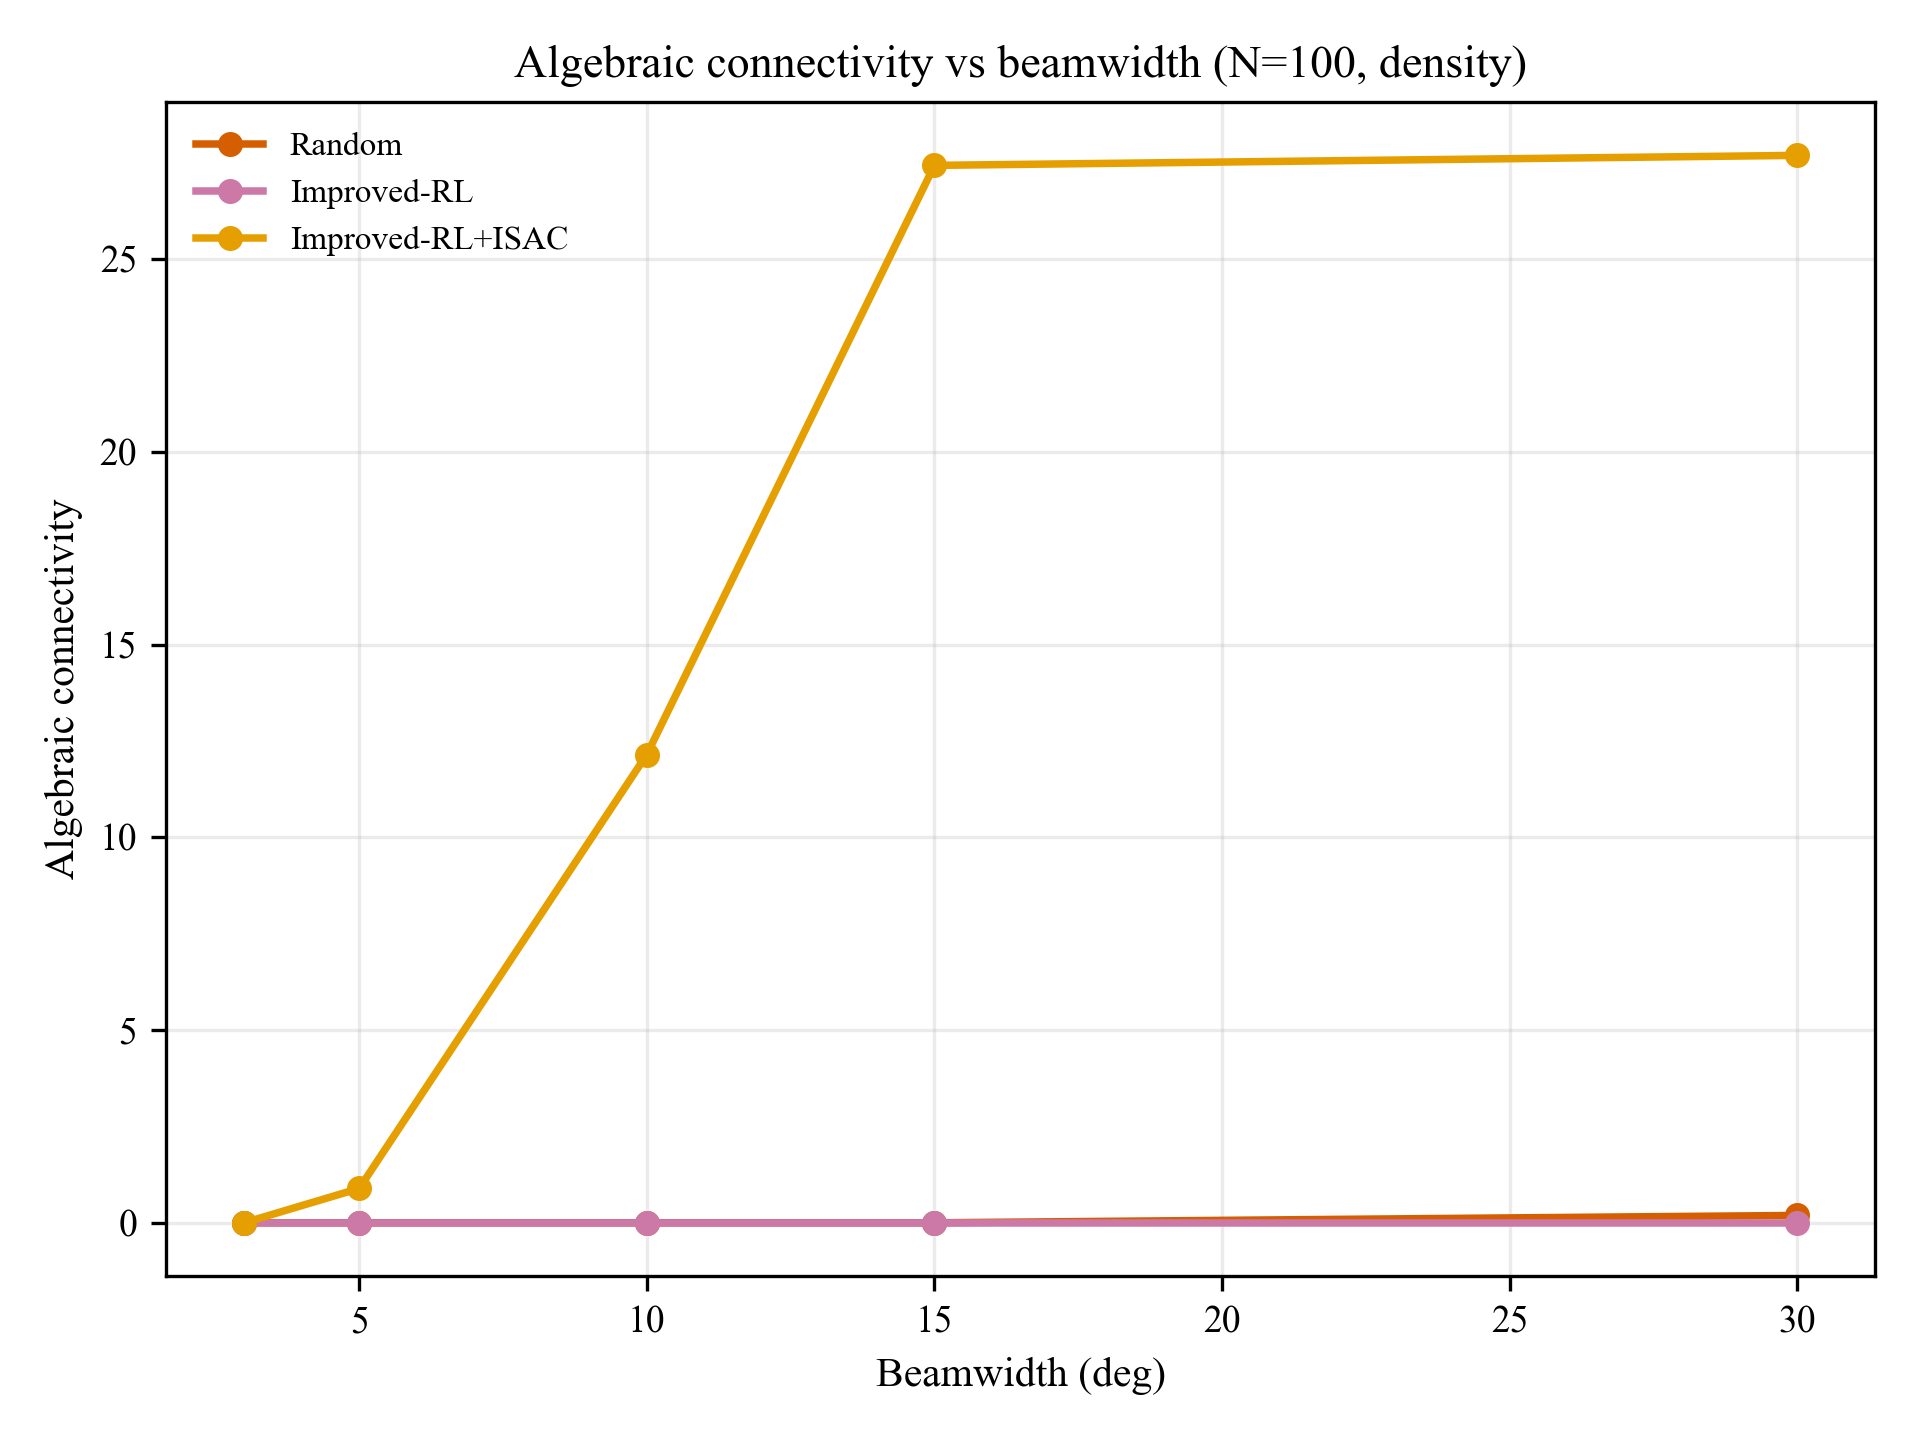
\includegraphics[width=0.32\textwidth]{../../06_analysis/paper_figures/round7_scale_beam_grid_light/density_beamwidth_lambda2_n100.png}
  \caption{N=100 beamwidth stress evidence. Left: raw discovery rate. Middle: collision-penalized discovery. Right: algebraic connectivity. The 3-degree and 5-degree points are stress regimes, while the 10--30 degree region provides the main useful operating range in the current finite horizon.}
  \label{fig:supp_beam_stress}
\end{figure*}

Table~\ref{tab:supp_b3} gives the targeted five-baseline check at $N=100$, 3-degree beams.
All baselines remain near zero, and the ISAC-assisted policy only reaches a small nonzero discovery rate.
This supports writing ``evaluated over 3--30 degrees,'' not ``effective over 3--30 degrees.''

\begin{table}[!t]
  \centering
  \caption{N=100, 3-Degree Five-Baseline Stress Check}
  \label{tab:supp_b3}
  \scriptsize
  \begin{tabular}{lcccc}
    \toprule
    Protocol & Disc. & Std. & Empty & $\lambda_2$ \\
    \midrule
    Uniform random & 0.0000 & 0.0000 & 0.9870 & 0.0000 \\
    SkyOrbs-like & 0.0000 & 0.0000 & 0.9865 & 0.0000 \\
    Learned no-ISAC & 0.0001 & 0.0001 & 0.9868 & 0.0000 \\
    Enhanced no-ISAC & 0.0000 & 0.0000 & 0.9871 & 0.0000 \\
    Enhanced ISAC & 0.0131 & 0.0007 & 0.9418 & 0.0000 \\
    \bottomrule
  \end{tabular}
\end{table}

\begin{figure*}[!t]
  \centering
  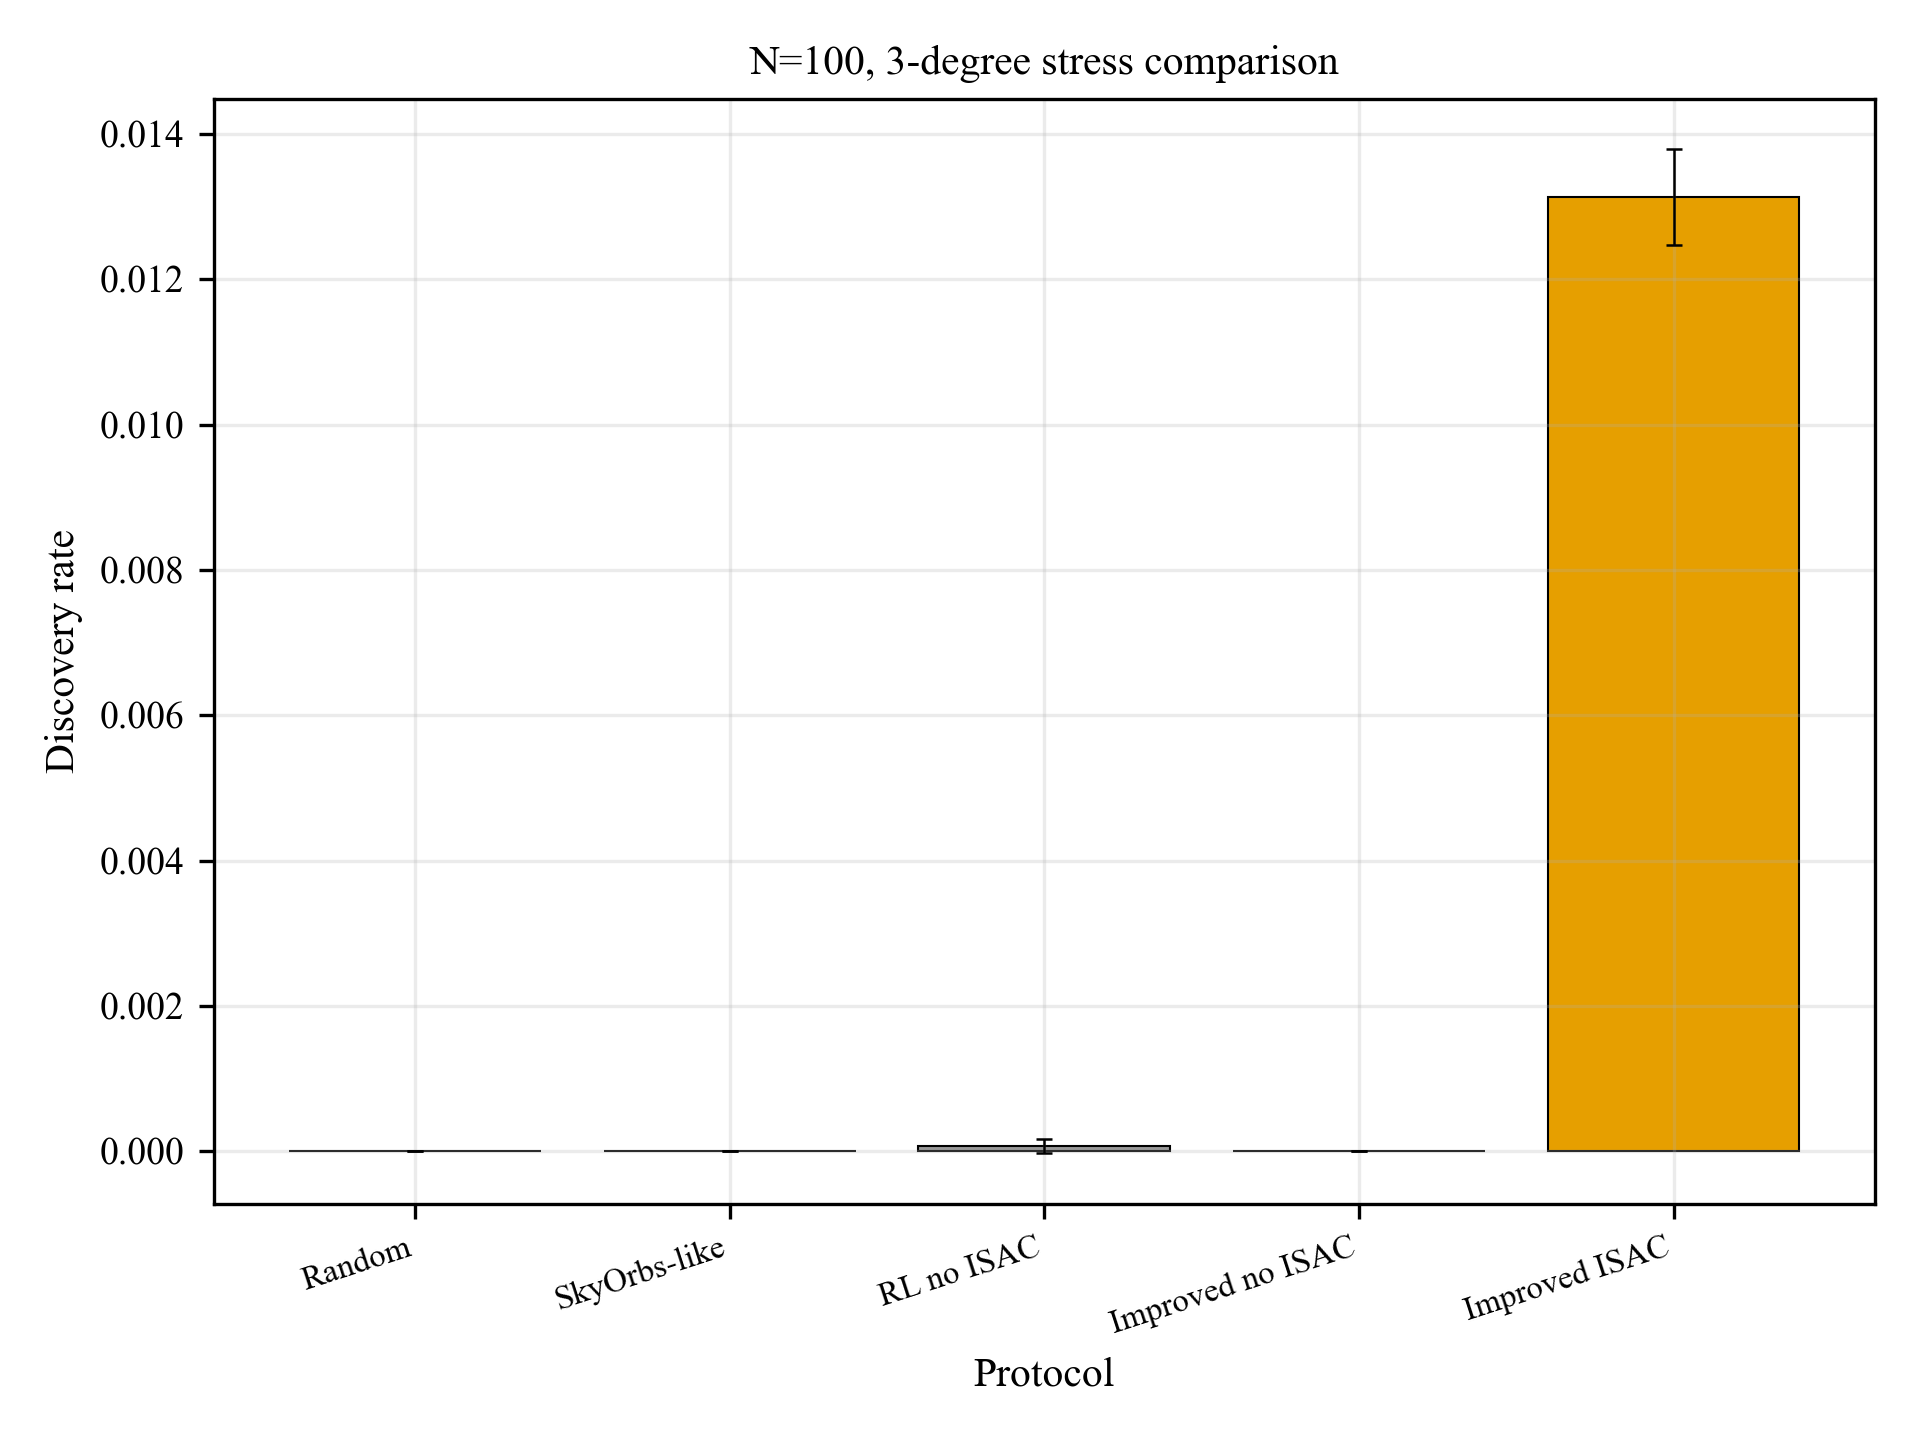
\includegraphics[width=0.48\textwidth]{../../06_analysis/paper_figures/round9_n100_b3_full_baselines_600slot/n100_b3_full_baselines_discovery.png}
  \hfill
  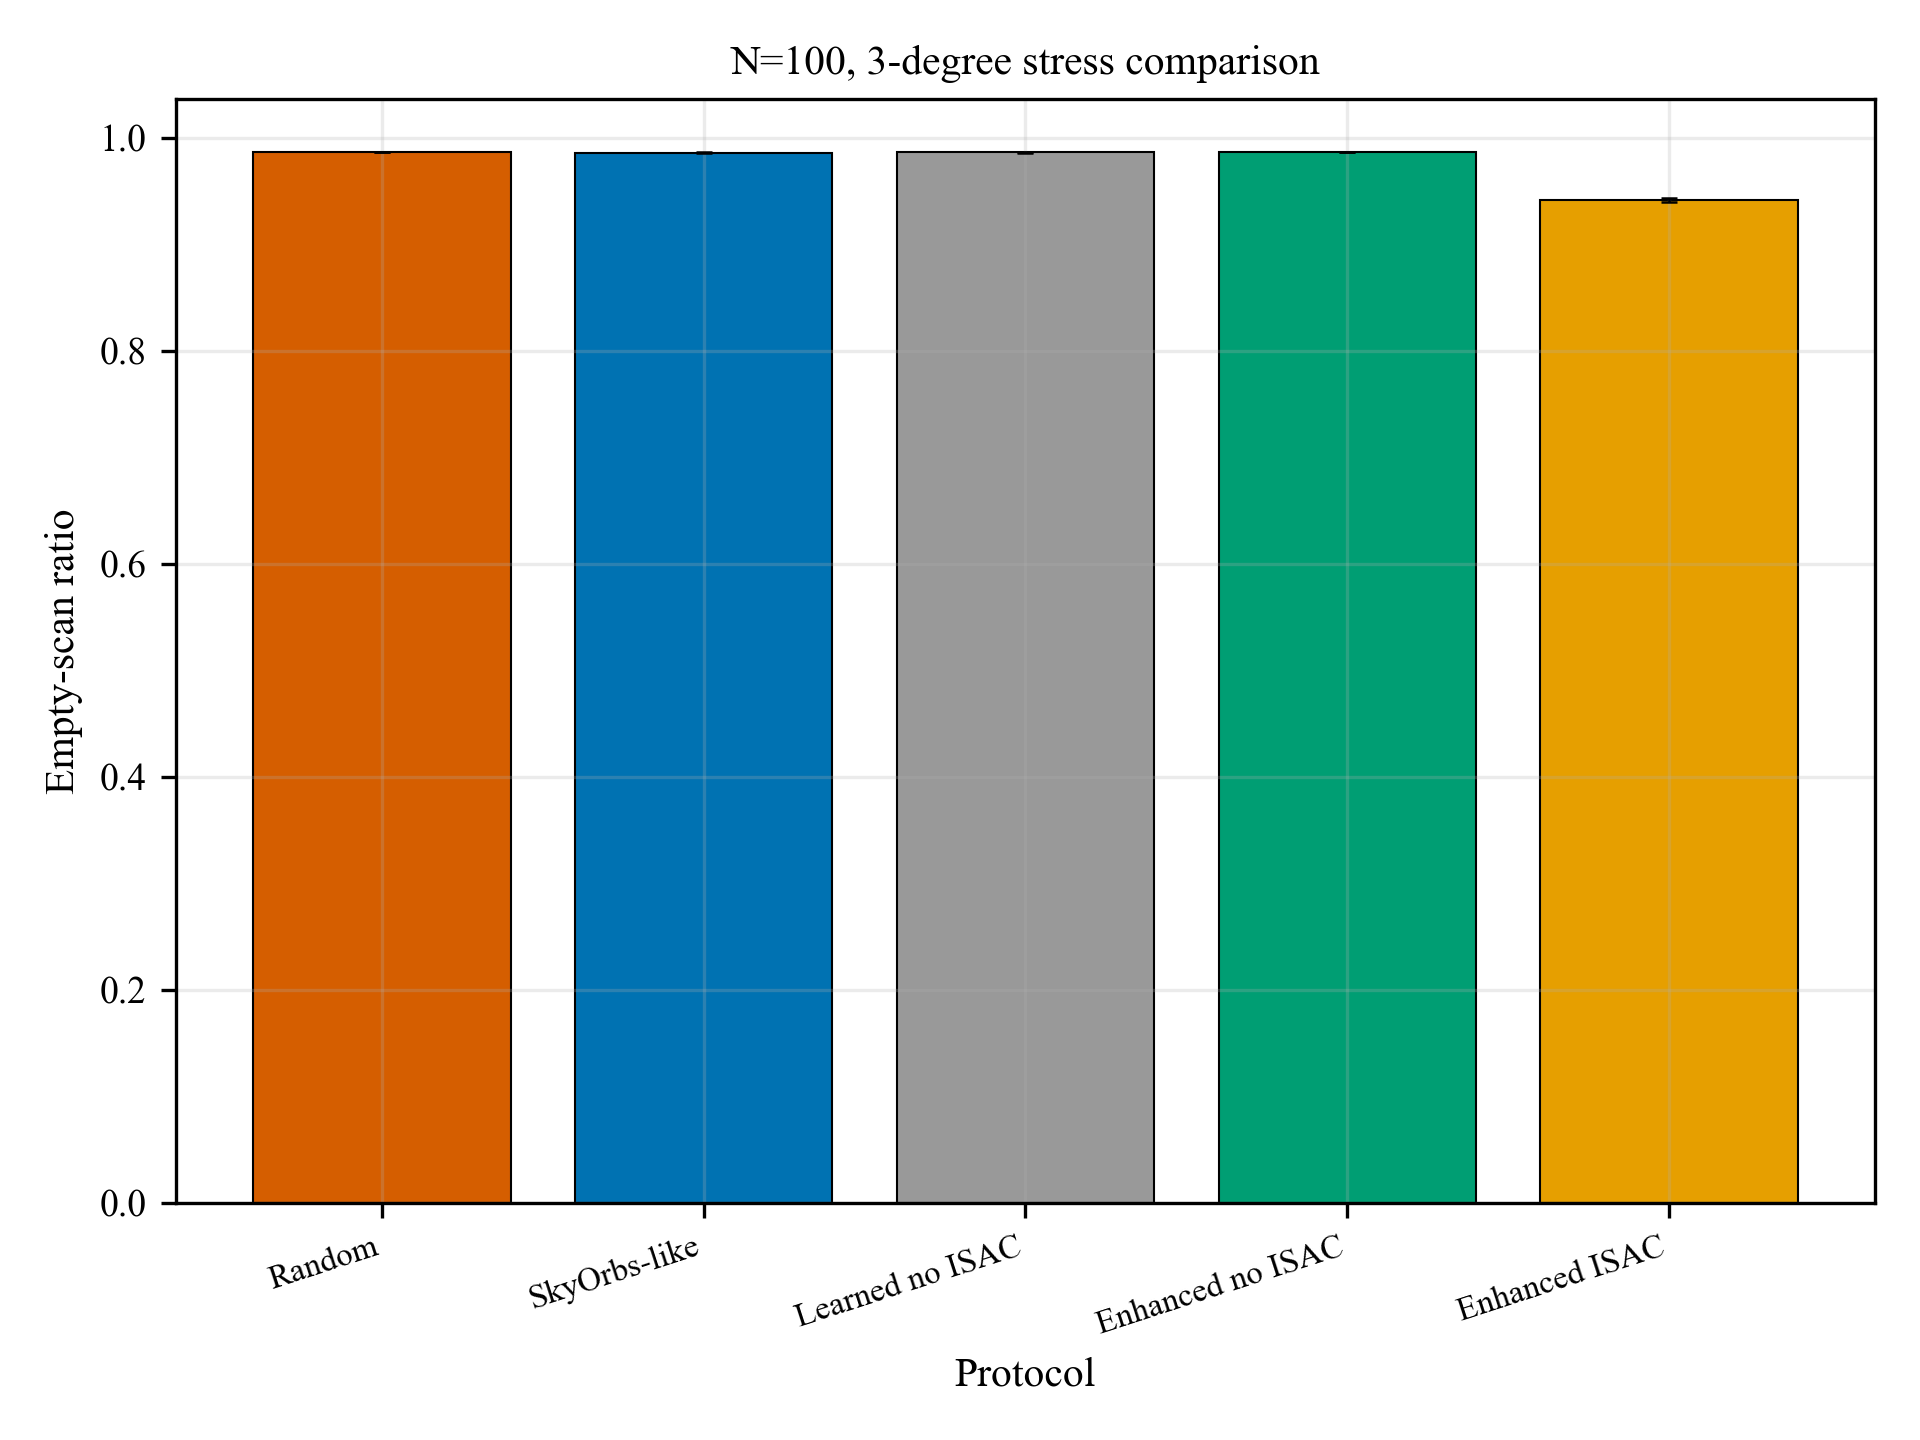
\includegraphics[width=0.48\textwidth]{../../06_analysis/paper_figures/round9_n100_b3_full_baselines_600slot/n100_b3_full_baselines_empty_scan.png}
  \caption{Full five-baseline comparison in the N=100, 3-degree stress case. Left: discovery rate. Right: empty-scan ratio. The plot is used as boundary evidence rather than main performance evidence.}
  \label{fig:supp_b3}
\end{figure*}

\section{Mobility Boundary and Missing Baselines}

Fig.~\ref{fig:supp_mobility_full} visualizes the merged round7/round8 mobility table.
It supports the mobility-boundary interpretation and indicates that the observed boundary is not caused by omitting the SkyOrbs-like or learned no-ISAC baseline.

\begin{figure*}[!t]
  \centering
  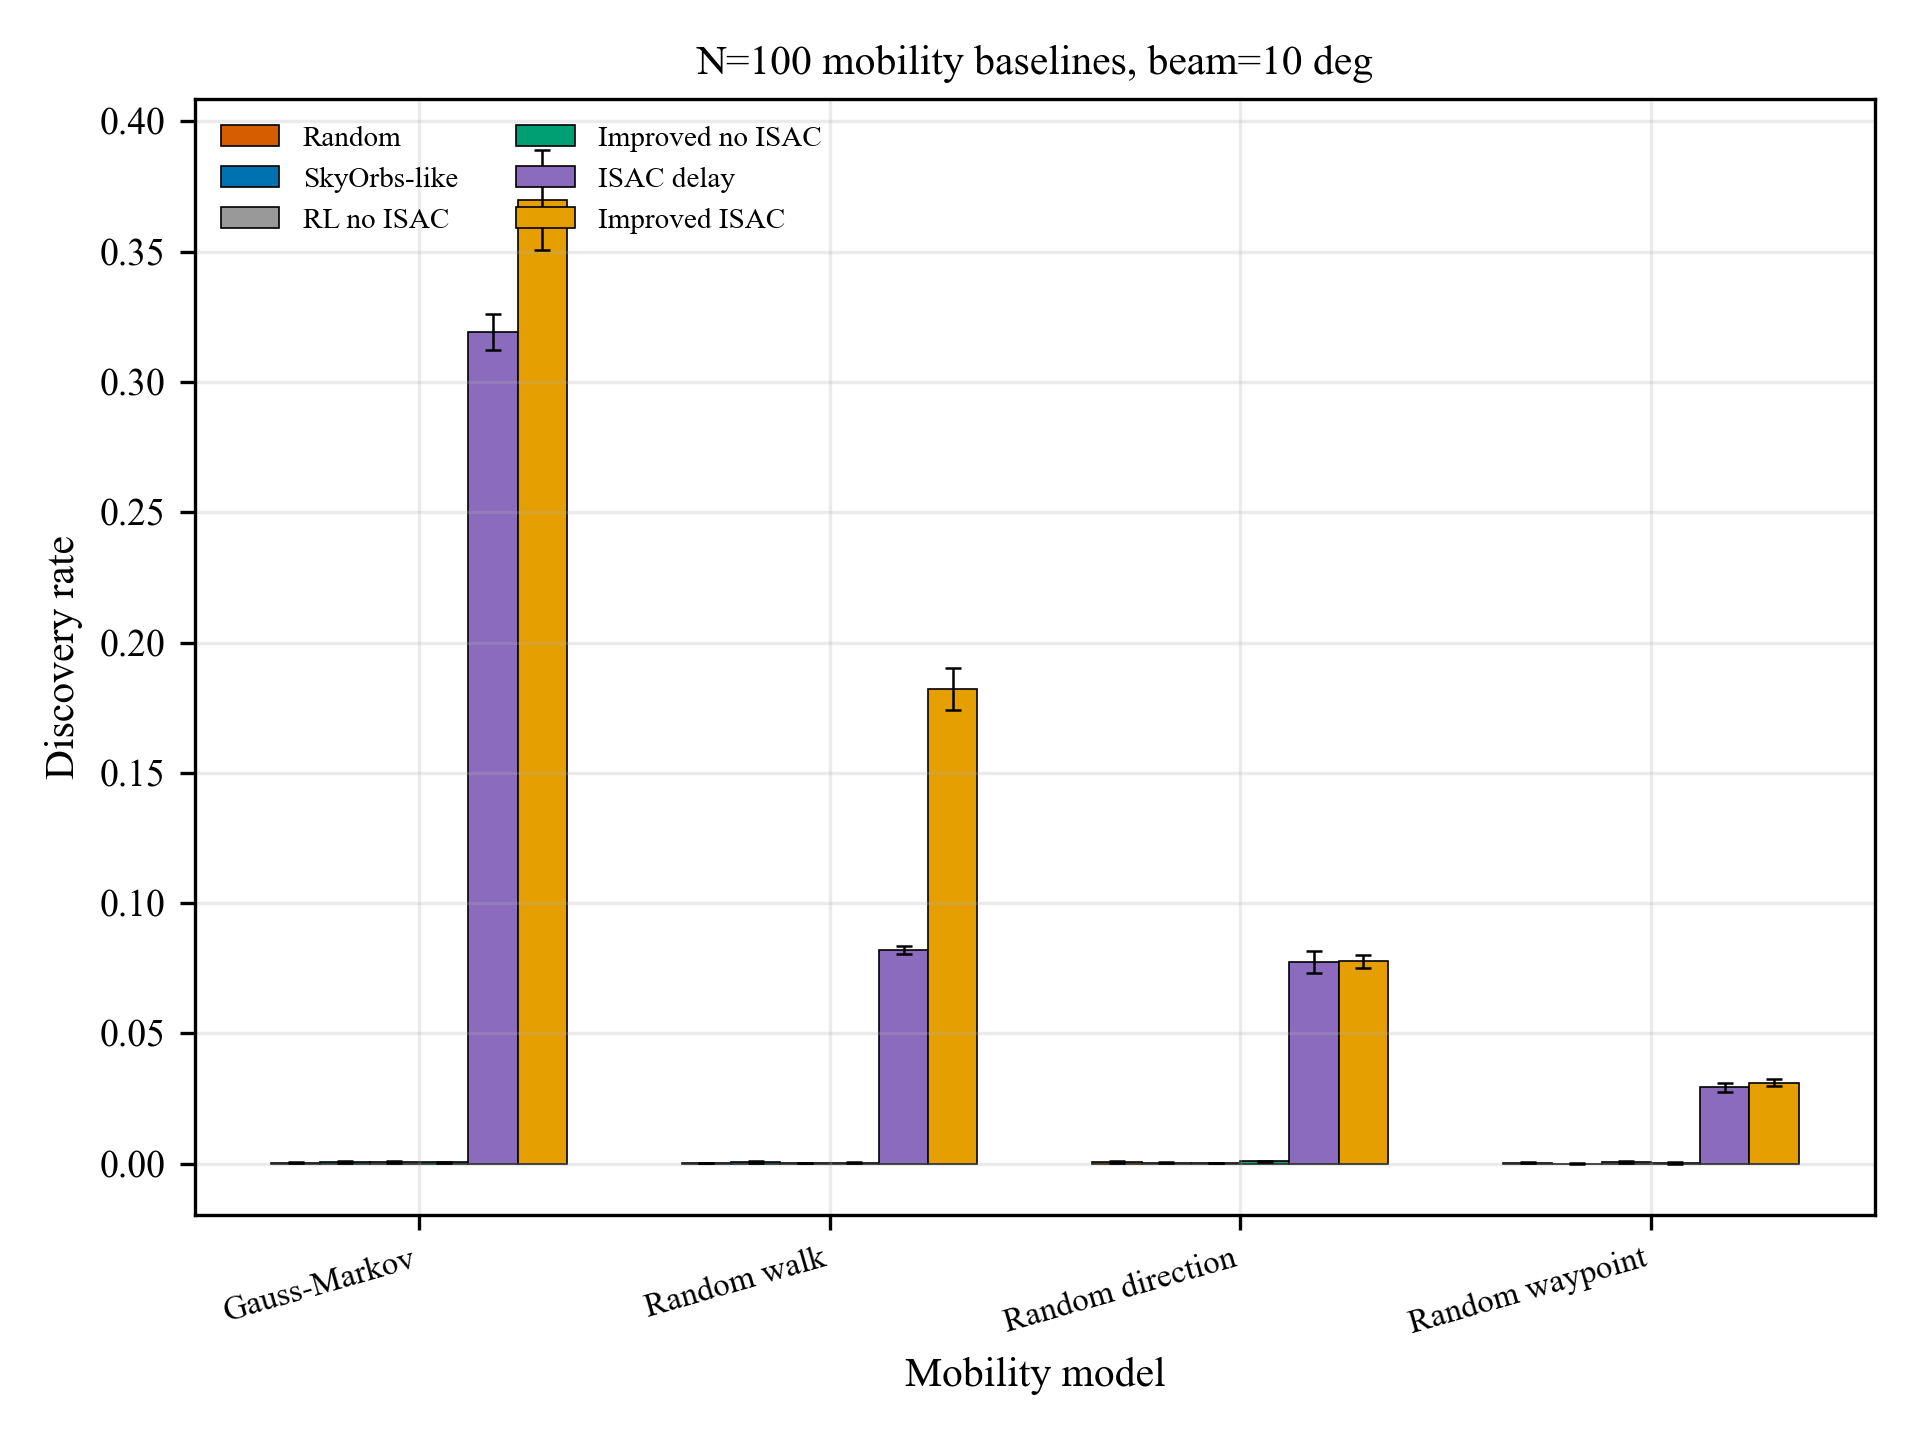
\includegraphics[width=0.48\textwidth]{../../06_analysis/paper_figures/round8_n100_multimobility_full_baseline/full_baseline_discovery_n100_b10.png}
  \hfill
  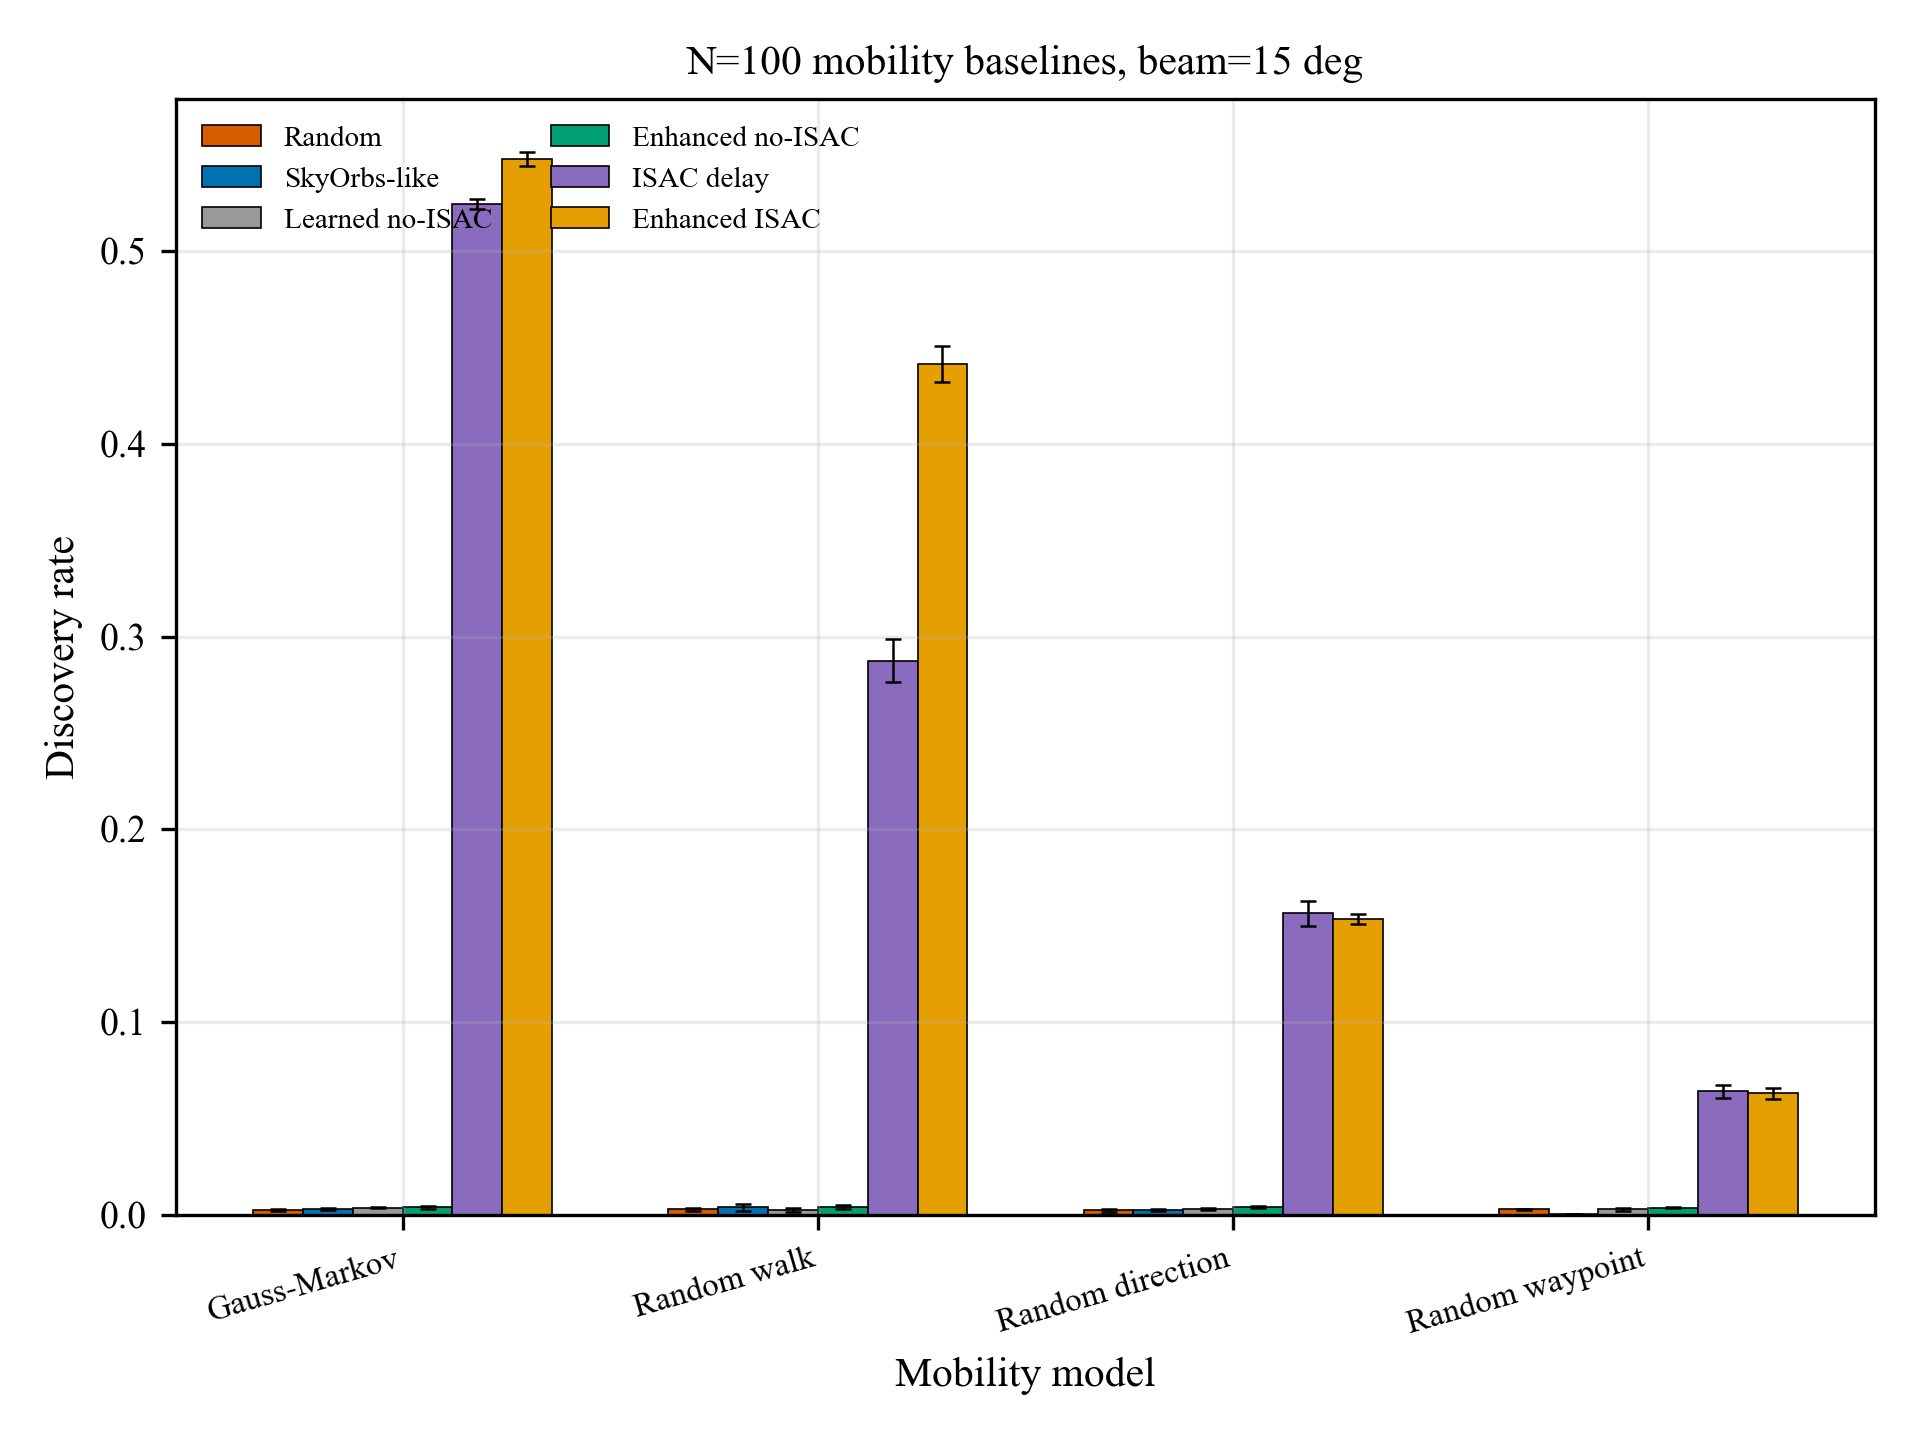
\includegraphics[width=0.48\textwidth]{../../06_analysis/paper_figures/round8_n100_multimobility_full_baseline/full_baseline_discovery_n100_b15.png}
  \caption{Full-baseline mobility comparison at N=100. Left: 10-degree beams. Right: 15-degree beams. The proposed ISAC-assisted policy has the highest observed discovery among the implemented baselines in these N=100, 10/15-degree mobility tests, while random-direction and random-waypoint remain stress regimes.}
  \label{fig:supp_mobility_full}
\end{figure*}

\section{B=15 Error Profiles}

The main paper reports B=10 sensing-error robustness.
Fig.~\ref{fig:supp_b15_error} extends the error-profile check to 15-degree beams and separates Gauss-Markov from random-walk mobility.
The key observation is that B=15 retains high raw discovery under Gauss-Markov but becomes more sensitive under random-walk mobility.

\begin{table}[!t]
  \centering
  \caption{Configured Protocol-Level ISAC Error Profiles}
  \label{tab:supp_error_profiles}
  \scriptsize
  \begin{tabular}{lccc}
    \toprule
    Profile & $P_{\mathrm{fa}}$ & $P_{\mathrm{md}}$ & Cell-offset std. \\
    \midrule
    Nominal & 0.00 & 0.00 & 0.0 \\
    Mild & 0.01 & 0.05 & 0.5 \\
    Moderate & 0.05 & 0.15 & 1.0 \\
    Severe & 0.10 & 0.30 & 1.5 \\
    \bottomrule
  \end{tabular}
\end{table}

\begin{figure*}[!t]
  \centering
  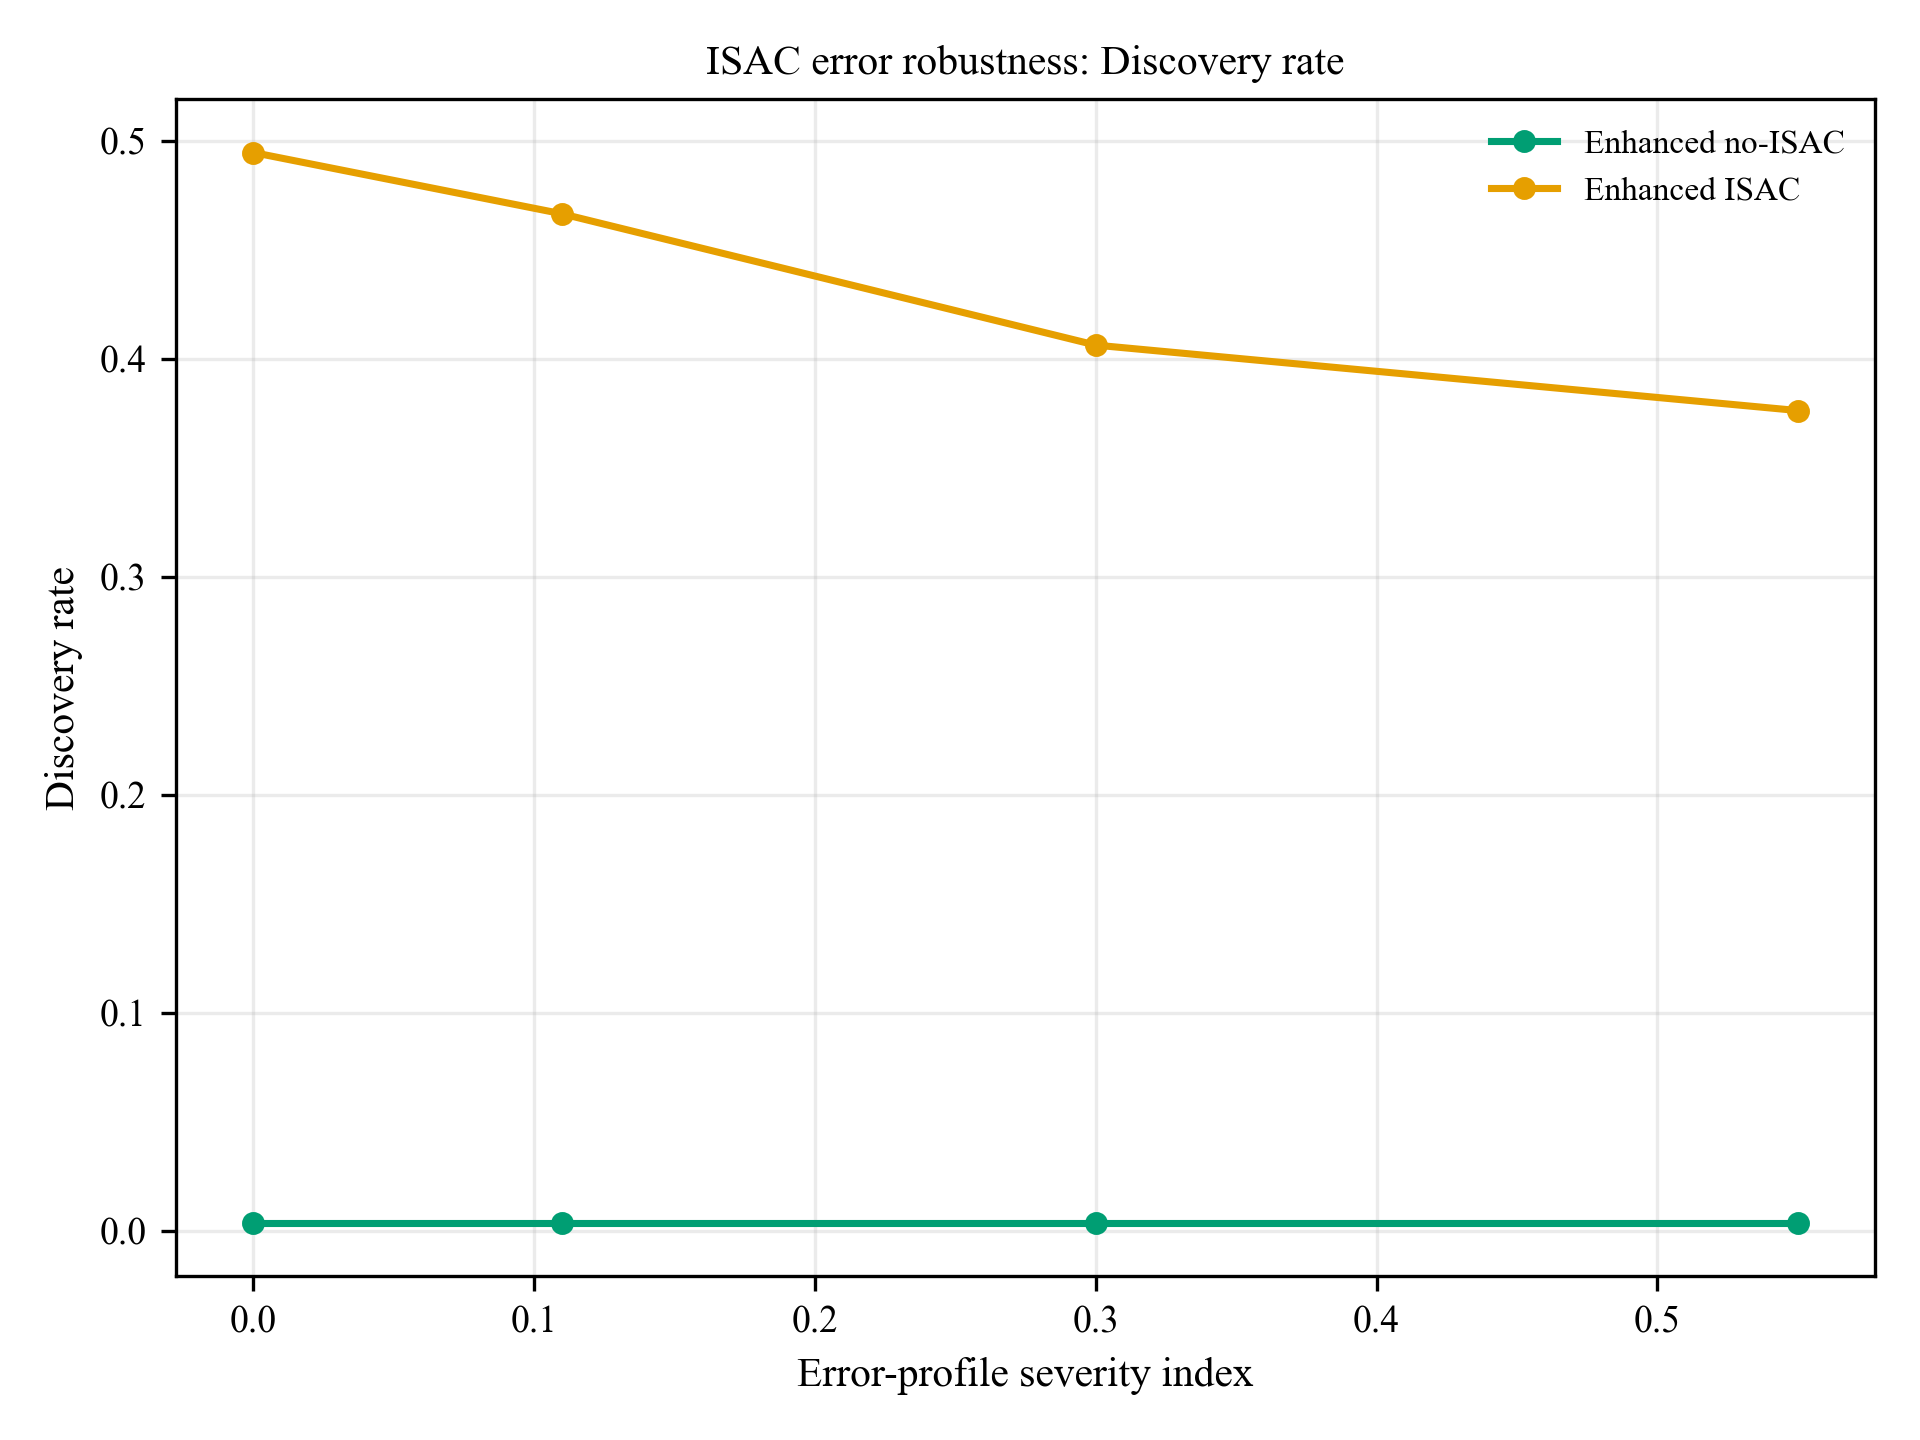
\includegraphics[width=0.48\textwidth]{../../06_analysis/paper_figures/round8_error_profiles_b15_gm_rw_600slot/error_profile_discovery_n100_b15.png}
  \hfill
  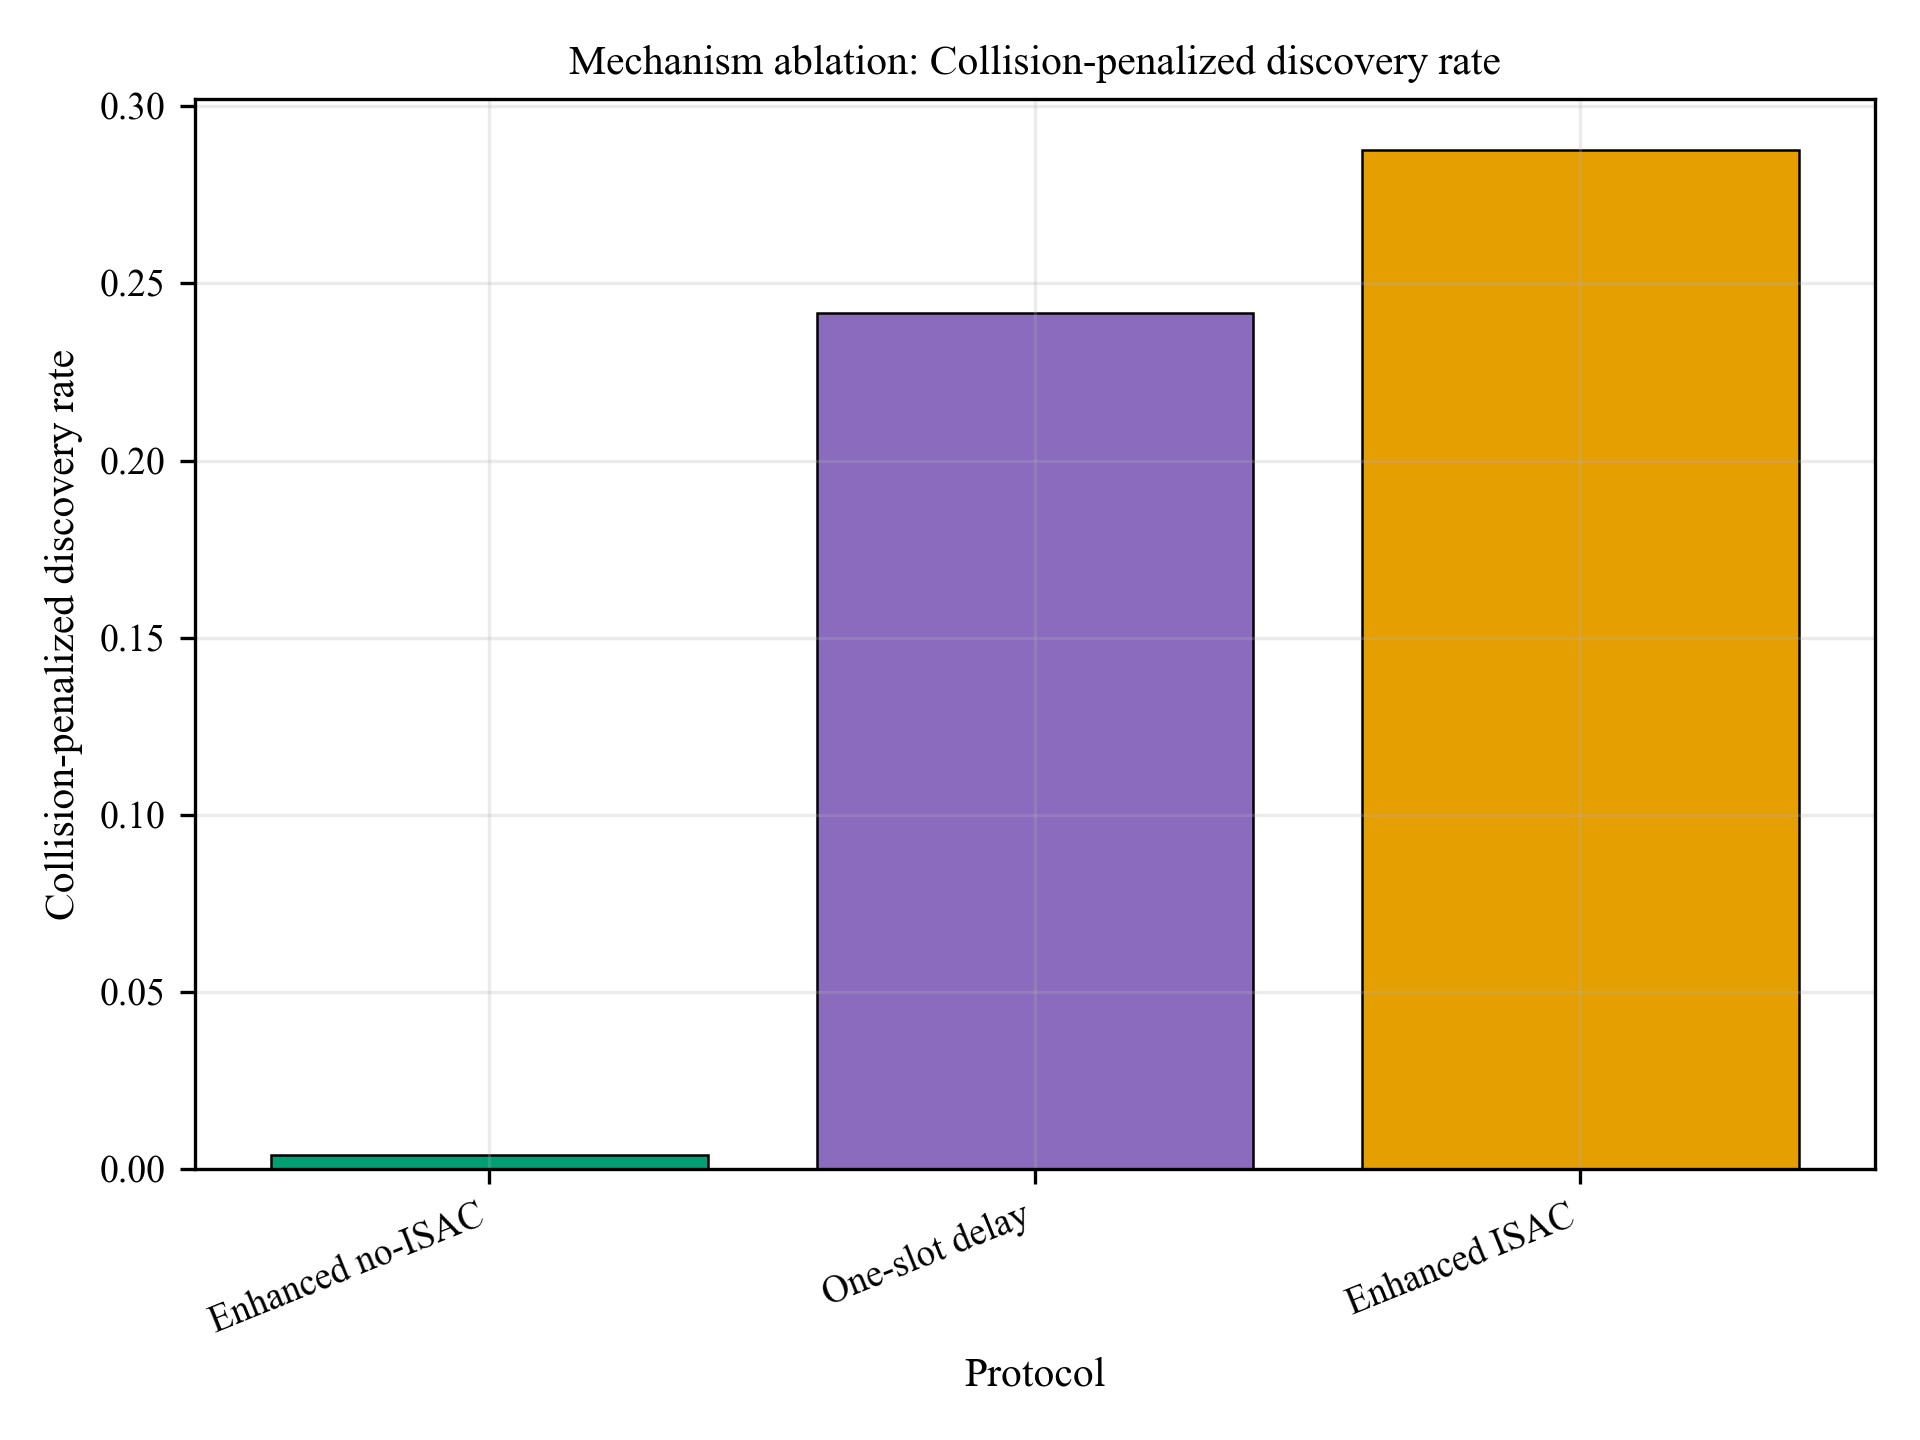
\includegraphics[width=0.48\textwidth]{../../06_analysis/paper_figures/round8_error_profiles_b15_gm_rw_600slot/ablation_collision_penalized_discovery_n100_b15.png}
  \caption{B=15 sensing-error extension. Left: raw discovery under configured ISAC error profiles. Right: collision-penalized mechanism-ablation comparison used to bound raw-discovery gains.}
  \label{fig:supp_b15_error}
\end{figure*}

\section{Reproducibility Notes}

All compact multi-seed summaries are archived under the repository paper-table directory.
The normalized statistical table is the \texttt{statistical\_stability\_summary.csv} artifact.
Rows tagged \texttt{main} support the manuscript tables and figures; rows tagged \texttt{main\_boundary}, \texttt{supplement}, or \texttt{supplement\_stress} should be used to bound claims and answer reviewer questions.
The statistical summary includes the N=10/20/50/100 scale-grid rows where archived, but many robustness and baseline-completeness checks are intentionally N=100-only.

\begin{table*}[!t]
  \centering
  \caption{Representative Multi-Seed Statistical Stability Checks}
  \label{tab:supp_stat_examples}
  \scriptsize
  \begin{tabular}{p{0.31\textwidth}cc}
    \toprule
    Scenario & Discovery mean$\pm$std (95\% CI) & $\lambda_2$ mean$\pm$std (95\% CI) \\
    \midrule
    N=100, B=10, density-scaled & 0.3655$\pm$0.0036 (0.0041) & 12.92$\pm$1.90 (2.15) \\
    N=100, B=15, density-scaled & 0.5440$\pm$0.0026 (0.0029) & 26.84$\pm$3.93 (4.45) \\
    N=100, B=3 stress & 0.0131$\pm$0.0007 (0.0007) & 0.00$\pm$0.00 (0.00) \\
    N=100, B=10, random walk & 0.2024$\pm$0.0086 (0.0097) & 5.95$\pm$0.50 (0.56) \\
    N=100, B=10, $\Rc/D=0.65$, $\Rs/\Rc=0.75$ & 0.3569$\pm$0.0042 (0.0047) & 13.20$\pm$1.13 (1.28) \\
    N=100, B=10, 20 ms slot & 0.3644$\pm$0.0155 (0.0175) & 13.24$\pm$1.17 (1.32) \\
    \bottomrule
  \end{tabular}
\end{table*}

\begin{table*}[!t]
  \centering
  \caption{Representative Paired Treatment-Control Deltas from Identical Scenario Seeds (n=3 Paired Seeds; Descriptive Bootstrap CI)}
  \label{tab:supp_paired_delta}
  \scriptsize
  \setlength{\tabcolsep}{3pt}
  \begin{tabular}{p{0.36\textwidth}ccc}
    \toprule
    Scenario and comparison & $\Delta$ discovery (descr. 95\% CI) & $\Delta$ empty or efficiency & $\Delta\lambda_2$ \\
    \midrule
    N=100, B=10, proposed vs enhanced no-ISAC & +0.3648 (0.3608, 0.3699) & Empty: -0.4025 & +12.92 \\
    N=100, B=15, proposed vs enhanced no-ISAC & +0.5403 (0.5370, 0.5428) & Empty: -0.5052 & +26.84 \\
    N=100, B=10, proposed vs candidate-set removal & +0.3341 (0.3297, 0.3416) & Coll.-penalized: +0.2702 & +12.92 \\
    N=100, B=10, one-slot delayed vs enhanced no-ISAC & +0.2982 (0.2891, 0.3133) & Coll.-penalized: +0.2613 & +8.47 \\
    N=100, B=10, random-walk proposed vs enhanced no-ISAC & +0.2021 (0.1899, 0.2101) & Empty: -0.1392 & +5.95 \\
    \bottomrule
  \end{tabular}
\end{table*}

\begin{table*}[!t]
  \centering
  \caption{Normalized Statistical Evidence Index}
  \label{tab:supp_stats_index}
  \scriptsize
  \begin{tabular}{p{0.20\textwidth}ccp{0.52\textwidth}}
    \toprule
    Tier & Rows & Episodes & Intended use \\
    \midrule
    \texttt{main} & 126 & 378 & Manuscript tables, range, error, and ablation claims. \\
    \texttt{main\_boundary} & 24 & 72 & Mobility-boundary evidence in the main paper. \\
    \texttt{supplement} & 156 & 408 & Scale-grid, beamwidth, mobility, and error extensions. \\
    \texttt{supplement\_backup} & 10 & 30 & Extra seed-sensitivity checks that bound, but do not replace, the main evidence. \\
    \texttt{supplement\_sanity} & 24 & 24 & Quick screens before full multi-seed checks. \\
    \texttt{supplement\_stress} & 5 & 15 & Targeted 3-degree full-baseline stress case. \\
    \bottomrule
  \end{tabular}
\end{table*}

The paired-delta table is generated from \texttt{paired\_delta\_summary.csv}; every row pairs protocols by identical scenario seeds and matching scenario parameters.
The intervals are descriptive bootstrap percentile intervals over paired seed-level deltas and should be interpreted together with the small number of seeds.

\end{document}
